%%%%%%%%%%%%%%%%%%%%%%%%%%%%%%%%%%%%%%%%%
% Journal Article
% LaTeX Template
% Version 1.4 (15/5/16)
%
% This template has been downloaded from:
% http://www.LaTeXTemplates.com
%
% Original author:
% Frits Wenneker (http://www.howtotex.com) with extensive modifications by
% Vel (vel@LaTeXTemplates.com)
%
% License:
% CC BY-NC-SA 3.0 (http://creativecommons.org/licenses/by-nc-sa/3.0/)
%
%%%%%%%%%%%%%%%%%%%%%%%%%%%%%%%%%%%%%%%%%

%----------------------------------------------------------------------------------------
%	PACKAGES AND OTHER DOCUMENT CONFIGURATIONS
%----------------------------------------------------------------------------------------

\documentclass[twoside]{article}
\usepackage{blindtext} % Package to generate dummy text throughout this template 

\usepackage[sc]{mathpazo} % Use the Palatino font
\usepackage[T1]{fontenc} % Use 8-bit encoding that has 256 glyphs
\linespread{1.05} % Line spacing - Palatino needs more space between lines
\usepackage{microtype} % Slightly tweak font spacing for aesthetics

\usepackage[english]{babel} % Language hyphenation and typographical rules

\usepackage[hmarginratio=1:1,top=32mm,columnsep=20pt]{geometry} % Document margins
\usepackage[hang, small,labelfont=bf,up,textfont=it,up]{caption} % Custom captions under/above floats in tables or figures
\usepackage{booktabs} % Horizontal rules in tables

\usepackage{lettrine} % The lettrine is the first enlarged letter at the beginning of the text

\usepackage{enumitem} % Customized lists
\setlist[itemize]{noitemsep} % Make itemize lists more compact
\usepackage{graphicx}
\usepackage{graphbox}
\usepackage{abstract} % Allows abstract customization
\renewcommand{\abstractnamefont}{\normalfont\bfseries} % Set the "Abstract" text to bold
\renewcommand{\abstracttextfont}{\normalfont\small\itshape} % Set the abstract itself to small italic text

\usepackage{titlesec} % Allows customization of titles
\renewcommand\thesection{\Roman{section}} % Roman numerals for the sections
\renewcommand\thesubsection{\roman{subsection}} % roman numerals for subsections
\titleformat{\section}[block]{\large\scshape\centering}{\thesection.}{1em}{} % Change the look of the section titles
\titleformat{\subsection}[block]{\large}{\thesubsection.}{1em}{} % Change the look of the section titles

\usepackage{fancyhdr} % Headers and footers
\pagestyle{fancy} % All pages have headers and footers
\fancyhead{} % Blank out the default header
\fancyfoot{} % Blank out the default footer
\fancyhead[C]{Running title $\bullet$ Nuvember 2022} % Custom header text
\fancyfoot[RO,LE]{\thepage} % Custom footer text
\usepackage{titling} % Customizing the title section
\usepackage{textcomp, gensymb}
\usepackage{subcaption}
\usepackage{float}

\usepackage{tikz}
\usetikzlibrary{shapes.geometric, arrows, chains}

\tikzstyle{startstop} = [rectangle, rounded corners, 
minimum width=3cm, 
minimum height=1cm,
text centered, 
draw=black, 
fill=red!30]

\tikzstyle{coord} = [
coordinate, 
node distance=2cm
]

\tikzstyle{io} = [trapezium, 
trapezium stretches=true, % A later addition
trapezium left angle=70, 
trapezium right angle=110, 
minimum width=3cm, 
minimum height=1cm, text centered, 
text width=3cm,
draw=black, fill=blue!30]

\tikzstyle{process} = [rectangle, 
minimum width=3cm, 
minimum height=1cm, 
text centered, 
text width=3cm,
draw=black, 
fill=orange!30]

\tikzstyle{decision} = [diamond, 
minimum width=4cm, 
minimum height=2cm, 
text centered, 
aspect=2,
draw=black, 
text width=3.5cm,
fill=green!30]

\tikzstyle{arrow} = [thick,->,>=stealth]
\usepackage[colorinlistoftodos]{todonotes}
\usepackage{hyperref} % For hyperlinks in the PDF
\graphicspath{{images/}}
\counterwithin{figure}{section}
\renewcommand{\thefigure}{\arabic{section}.\arabic{figure}}

\counterwithin{table}{section}
\renewcommand{\thetable}{\arabic{section}.\arabic{table}}

%----------------------------------------------------------------------------------------
%	TITLE SECTION
%----------------------------------------------------------------------------------------

\setlength{\droptitle}{-4\baselineskip} % Move the title up

\pretitle{\begin{center}\Huge\bfseries} % Article title formatting
\posttitle{\end{center}} % Article title closing formatting
\title{Article Title} % Article title
\author{%
\textsc{Ethan Hu}\thanks{A thank you or further information} \\[1ex] % Your name
\normalsize ... \\ % Your institution
\normalsize \href{mailto:...}{...} % Your email address
%\and % Uncomment if 2 authors are required, duplicate these 4 lines if more
%\textsc{Jane Smith}\thanks{Corresponding author} \\[1ex] % Second author's name
%\normalsize University of Utah \\ % Second author's institution
%\normalsize \href{mailto:jane@smith.com}{jane@smith.com} % Second author's email address
}
\date{\today} % Leave empty to omit a date
\renewcommand{\maketitlehookd}{%
\begin{abstract}
\noindent 
	Soft-body robots have always received less attention compared to other branches of robotics. However, this does not suggest that they are any less capable than traditional robots due to their extreme flexibility. Soft robots commercially can be used in medical situations and with human interaction. This includes deployment into a human's body. However, the use case also extends into disaster relief situations. The flexibility of soft robots gives them an advantage over rigid robots when they are navigating through narrow spaces. Because of this flexibility, designing an optimized and sturdy system is difficult. In this paper, I proposed a new soft-body snake that is more optimized for real-life situations.
	The goal of this study is to create a better version of the soft robotic snakes already developed. This can be divided into two parts: software, and hardware. The software part would include software on the robot, and software on the computer. The micro controller on the robot would need to process images with Machine Learning and Vision to better identify the environment. The robot also identifies objects and obstacles around it and sends their positions along with the video from the camera and some other data such as humidity and temperature altogether back to the computer. The computer then constructs a 3D map of the area and outputs the video to the user. The user can also choose to control the robot manually and the computer would send these commands to the robot. 
	The goal for the hardware part of the robot is to implement a more efficient flexible structure that better utilizes the air pressure and moves more controllably. The structures previous soft robotic snakes utilize is requires high air pressure and the expansion is rather uncontrolled and unideal. The structure is also very complicated and the connection between the flexible and rigid parts is hard to work with, not to mention the difficulties with preventing leakage of air with those structures.
\end{abstract}
}

%----------------------------------------------------------------------------------------

\begin{document}

% Print the title
\maketitle

%----------------------------------------------------------------------------------------
%	ARTICLE CONTENTS
%----------------------------------------------------------------------------------------

\section{Introduction}
\subsection{Background}
\lettrine[nindent=0em,lines=3]{E} very second counts after a disaster yet rescue teams cannot always get to places needing the most help right away due to obstacles and often dangers. This could include collapsed buildings, flooded tunnels, ablaze rooms, etc. To shorten the time between the disaster providing aid, mere human isn’t enough. Specialized robots for different deadly environments are needed to support the rescue effort better. 
Collapsed buildings can be seen anywhere after almost all types of disasters — earthquakes, hurricanes, tsunamis, etc. Clearing a path through tons of debris is both time-consuming and laborious. To explore this environment more efficiently and more easily, a much smaller robot, and much more suited for this situation is needed — a soft robotic snake. Bionic snakes are naturally perfect for slithering through tight gaps and small tubes that the rescuers would otherwise be unable to cross. This could drastically speed up the exploration of ruined areas and the time takes to get to the ones needing help. Although this cannot fully replace the purpose of human rescuers and the need to clear up the area to people, this can provide some emergent aid while the main rescue force is on its way. 

\begin{figure}
\centering
\begin{subfigure}[b]{0.45\linewidth}
	\centering
	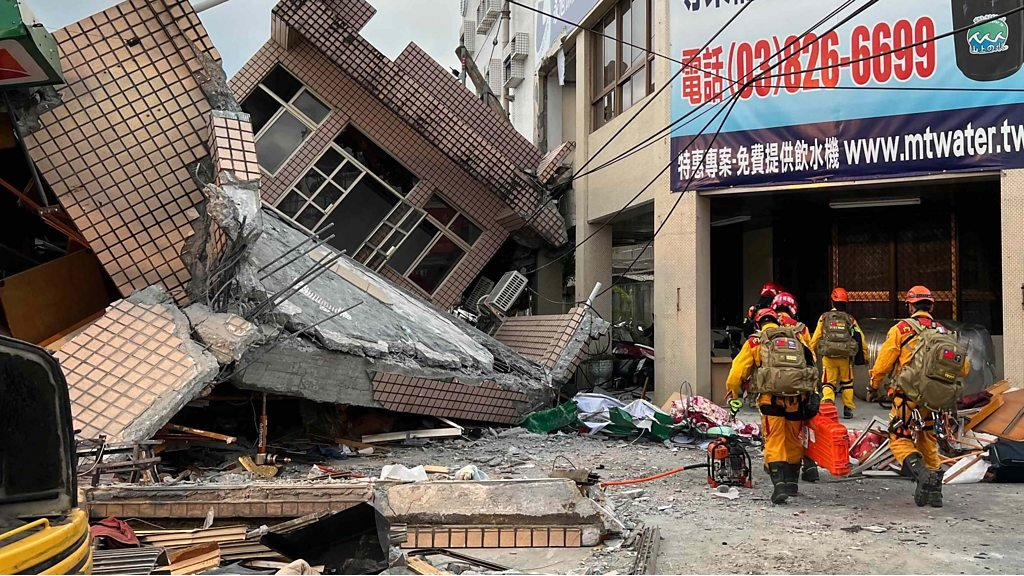
\includegraphics[width=\textwidth]{ruins}
	\subcaption{Collapsed building after earthquake can be especially dangerous for rescuers}
\end{subfigure}
\begin{subfigure}[b]{0.45\linewidth}
	\centering
	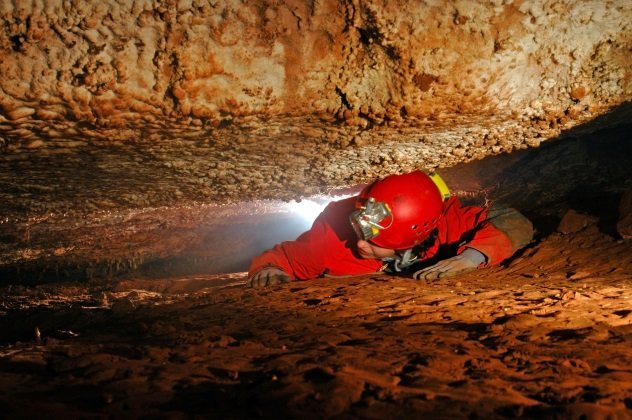
\includegraphics[width=\textwidth]{narrow passage}
	\subcaption{Some narrow passages are so small that rescuers cannot fit through}
\end{subfigure}
\caption{Examples of imagined usecases}
\end{figure}

\subsection{Current Studies}
This life-saving robot is of course not a completely new area of study. Many researchers have already attempted to recreate this fascinating animal. Wright and his team developed a simple modular robotic snake design using chained servos. Crespi and his team developed a more complicated robotic snake involving DC motors and detachable wheels to traverse both on the ground and in water. However, rigid bodies cannot fully mimic the movement of snakes as these robots can only move at the joints. Thus, many turned to softer and more flexible materials to achieve smoother turns. In a report presented at the International Conference of Soft Robotics (RoboSoft), Qin and his team used silicon tubes to achieve segments with 3 degrees of freedom (DoF). Each tube is responsible for 1 DoF and with three tubes, the soft robotic snake can perform locomotion much closer to that of a real snake than the rigid robotic snake. However, their design is much more complicated than the ones previously mentioned, as flexible material and air pressure are much harder to work with than rigid material and pulse-width modulation (PWM) signals. Apart from the production difficulties this design also lacks a more autonomous control system and a real-time feedback system that is crucial to its real-world applications. 

%------------------------------------------------

\section{Theoretical Design}
\subsection{Design Mentality}
As a soft-body robot, it has both flexible and rigid parts. Therefore, I split the designing task into two parts and approached them independently. I first worked on the flexible structures, which are the moving parts, and then designed the rigid structures holding the flexible structures in place and connecting them together. After finishing the general structure of the robot, I then added the electrical components to it.

\begin{figure}[H]
	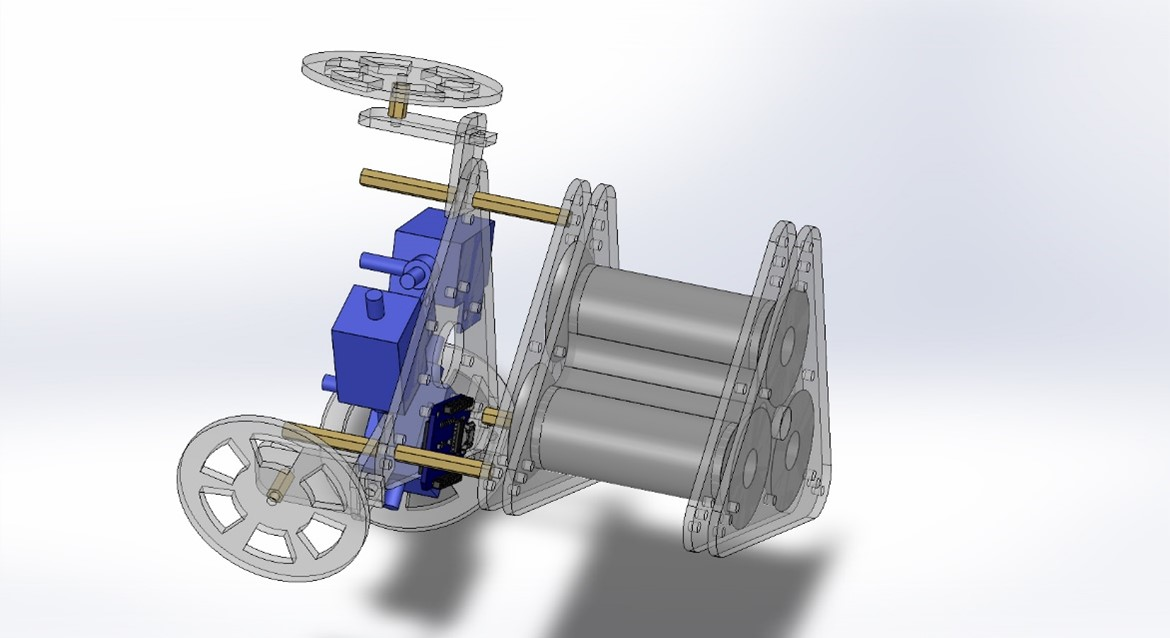
\includegraphics{overall_structure}
	\centering
	\caption{A complete segment of the snake}
\end{figure}

\subsection{Snake Locomotions}
\blindtext
\todo{talk about different ways the snake move, explain how it is replicated, friction, etc}

\subsection{Flexible Structures}
Rubber silicon was the ideal material for the flexible part as it is accessible elastic, and malleable, which is important for this project as all flexible parts are non-standard and require special molds. Between all the firmness of the rubber silicon, Shore A-10 was determined to be the best hardness as it retains the shape well without pressure and is still soft enough to deform under high air pressure. The original design of the silicon part is that it will have three hollow tubes connected in a triangular pattern. However, this was proven to be ineffective as it would detach from the silicon part when the chamber expands. Each tube will be then sealed on both ends with a tubing that allows the air pump to expand the chamber. A spring was designed to be around the bore in hopes of constraining the expansion to vertical only and preventing outward expansion. There will be a ring around each end of the tubes to allow a firm seal between the silicon part and the acrylic pieces used to secure the silicon parts.  

\begin{figure}[H] 
	\centering
	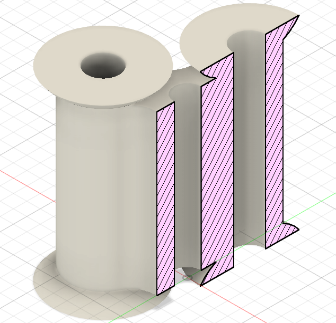
\includegraphics[scale=0.75]{silicon_body_half}
	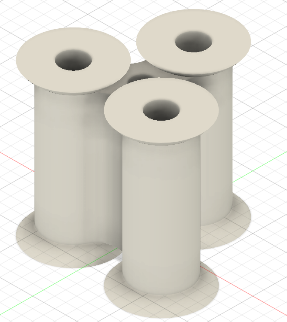
\includegraphics[scale=0.75]{silicon_body}
	\caption{The shape of the silicon body}
\end{figure}
\begin{figure}[H]
	\centering
	\begin{minipage}{0.45\textwidth}
		\centering
		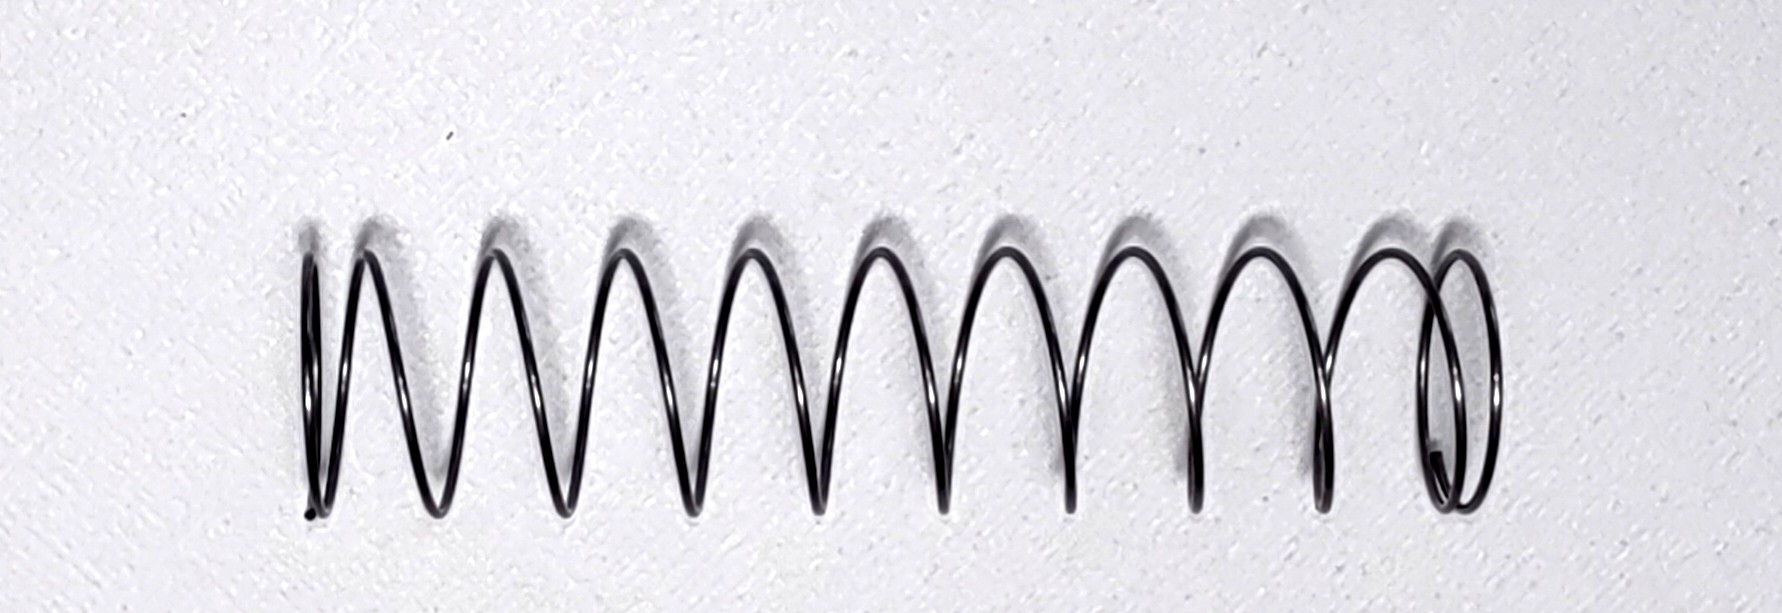
\includegraphics[angle=-90]{spring}
		\caption{spring used in the silicon part}
	\end{minipage}
	\hfill	
	\begin{minipage}{0.45\textwidth}
		\centering
		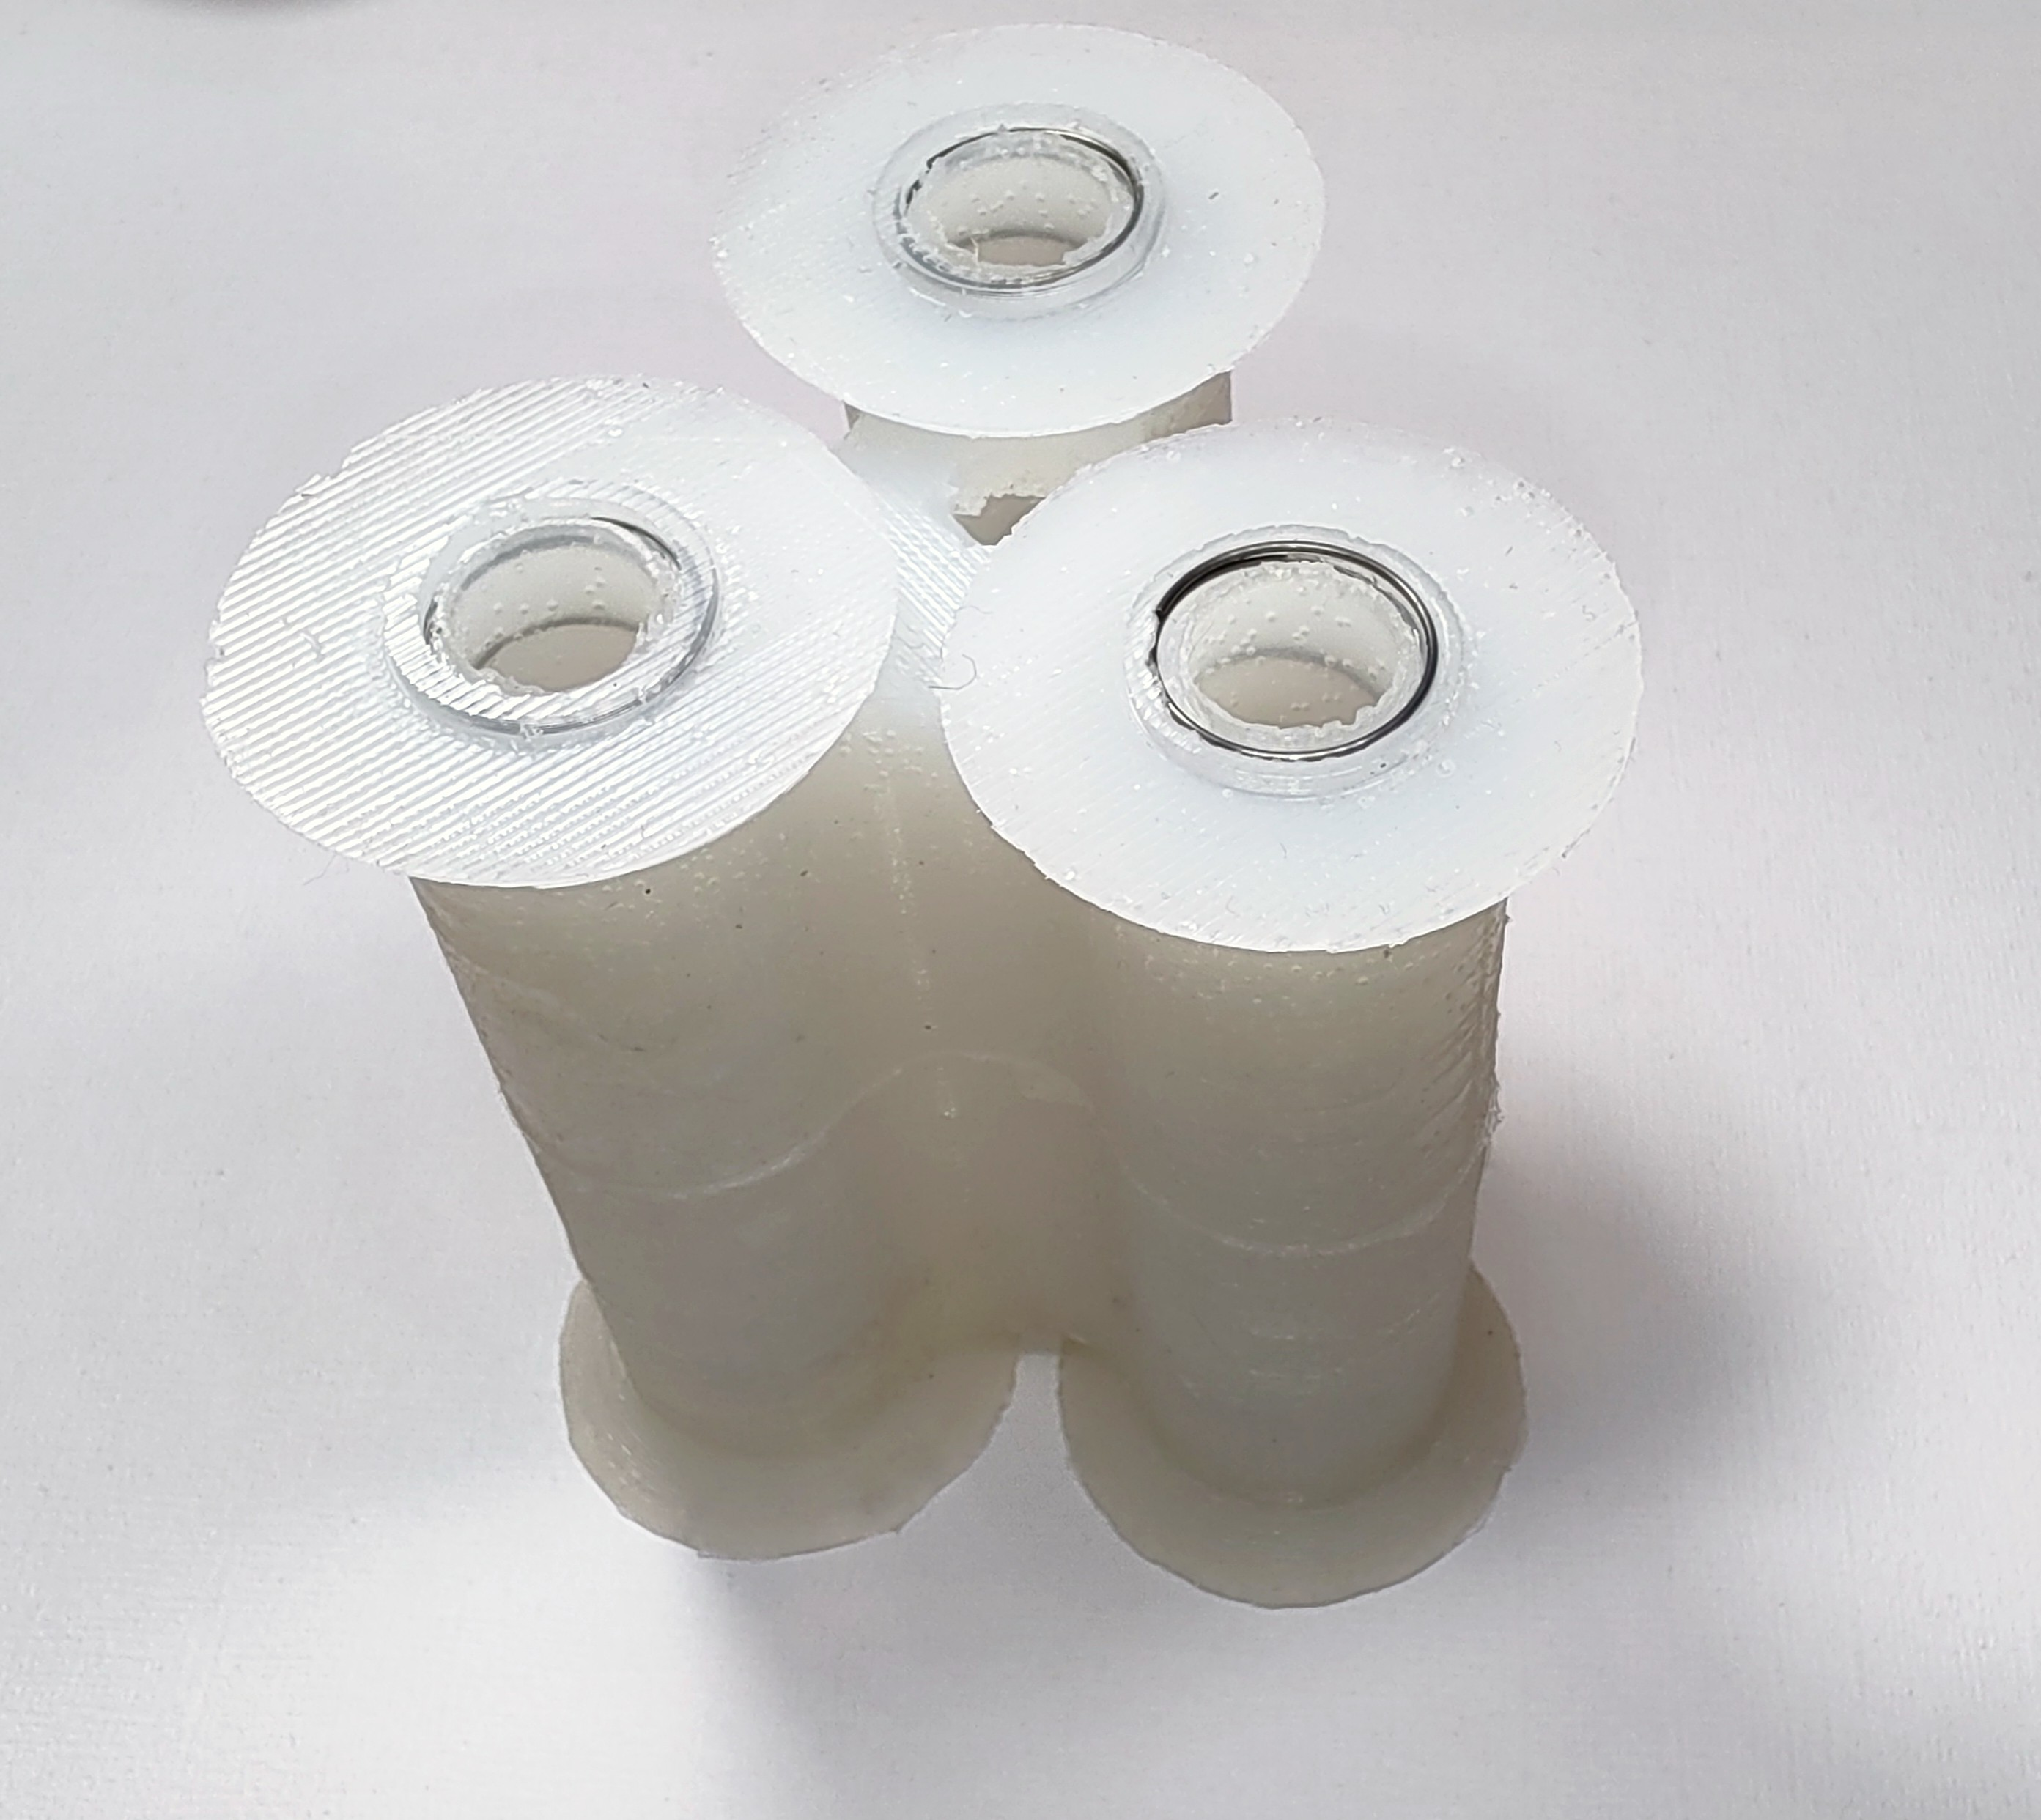
\includegraphics{silicon_with_spring}
		\caption{the silicon part with embedded spring}
	\end{minipage}
\end{figure}

\subsection{Rigid Structure}
The rigid structures are going to be made of acrylic as it is both a strong material and can be easily processed by my CNC router. There will be two pieces of acrylic on each side of the silicon part to secure it in place, and one end will house the air valve and the electronics. Each silicon part will be independent of the others to ensure modularity.

\begin{figure} [H]
	\centering
	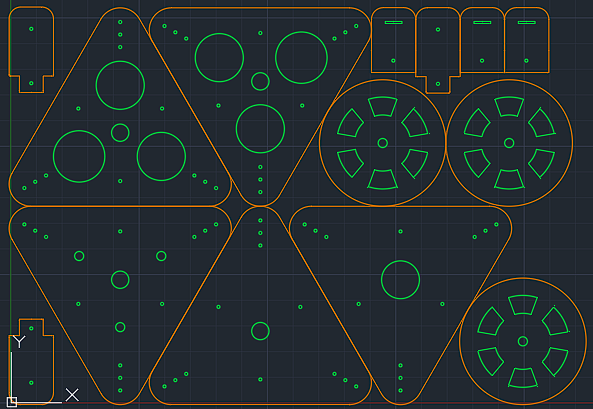
\includegraphics[scale=0.5]{acrylic_plate_cad}
	\caption{CAD file of the acrylic plates}
\end{figure}

\subsection{Silicon Body Parameters}
Before making any molds and actual parts, I wanted to test different wall thicknesses and inner diameters to find one that is most ideal for my use case. I used Simulia Abaqus to simulate the results to ensure that all variables are controlled, and only the independent variable changes. The First experiment is to determine the best wall thickness. For this, I chose three different thicknesses, 4mm, 5mm, and 6mm with a uniform diameter of 15mm. I predicted that the thinner the wall is, the larger the angle gets, which matched the actual results from the simulation.

\begin{table} [H]
	\centering
	\begin{tabular}{|c|c|c|c|c|}
	\hline
	Wall Thickness (mm) & $T_{1}$ Angle (\degree) & $T_{2}$ Angle (\degree) & $T_{3}$ Angle (\degree) & $T_{4}$ Angle (\degree)\\
	\hline
	4 & 22.5 & 32.07 & 41.36 & 42.7\\
	\hline
	5 & 18.96 & 29.8 & 34.22 & 36.98\\
	\hline
	6 & 4.96& 19.85 & 24.18 & 29.9\\
	\hline
	\end{tabular}
	\caption{The angle of the silicon arts with various wall thicknesses at different times of simulation}
\end{table}

\begin{table} [H]
	\centering
	\begin{tabular}{|c|c|}
	\hline
	Wall Thickness (mm) & largest Angle (\degree)\\\hline
	4 & 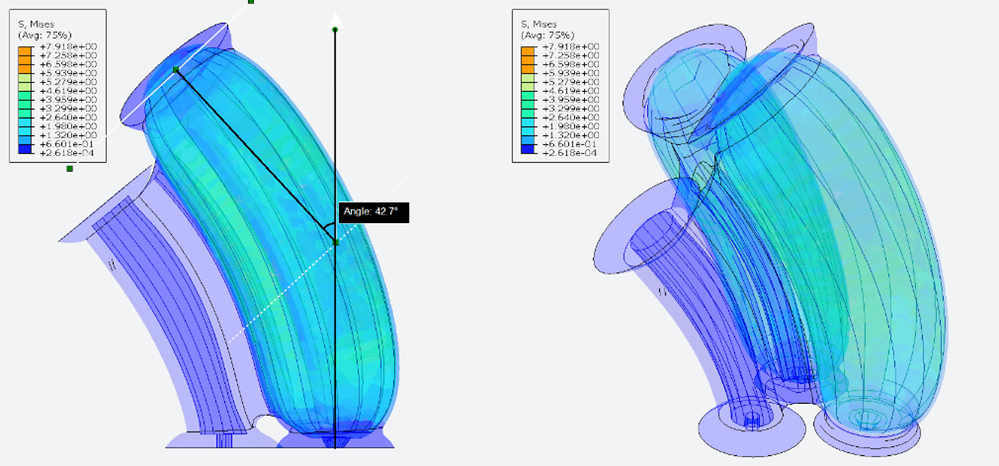
\includegraphics[align=c, scale=0.75]{wall4}\\\hline
	5 & 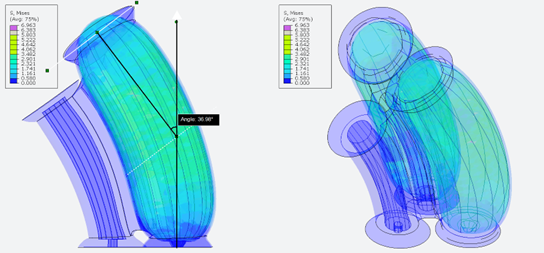
\includegraphics[align=c, scale=0.75]{wall5}\\\hline
	6 & 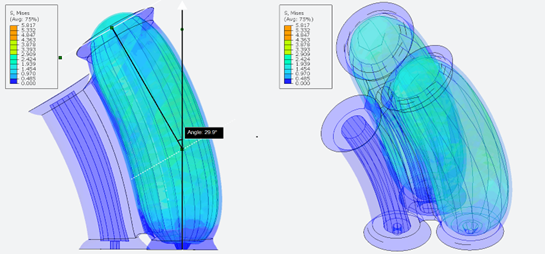
\includegraphics[align=c, scale=0.75]{wall6}\\\hline
	\end{tabular}
	\caption{The final angle after the silicon is fully inflated}
\end{table}

Then, I tested the effect of inner diameter on the max angle the part can bend. I predicted that the angle is inversely proportional to the diameter as a larger diameter result in a larger surface area, and thus the pressure is more spread out and can deform the silicon less. Turns out the hypothesis was partially correct. While the 14mm starts with smaller angles, it has the largest angle.

\begin{table} [H]
	\centering
	\begin{tabular}{|c|c|c|c|c|}
	\hline
	Chamber Diameter (mm) & $T_{1}$ Angle (\degree) & $T_{2}$ Angle (\degree) & $T_{3}$ Angle (\degree) & $T_{4}$ Angle (\degree)\\
	\hline
	14 & 10.55 & 23.43 & 33.64 & 38.88\\
	\hline
	15 & 	18.96 & 	29.8 & 	34.22	 & 36.98\\
	\hline
	16	 & 21.42	 & 29.31	 & 34.24	 & 34.93\\
	\hline
	\end{tabular}
	\caption{The angle of the silicon parts with various inner diameters at different times of simulation}
\end{table}

\begin{table} [H]
	\centering
	\begin{tabular}{|c|c|}
	\hline
	Wall Thickness (mm) & largest Angle (\degree)\\
	\hline
	4 & 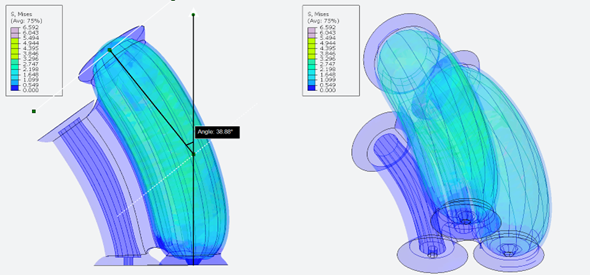
\includegraphics[align=c, scale=0.75]{d14}\\
	\hline
	5 & 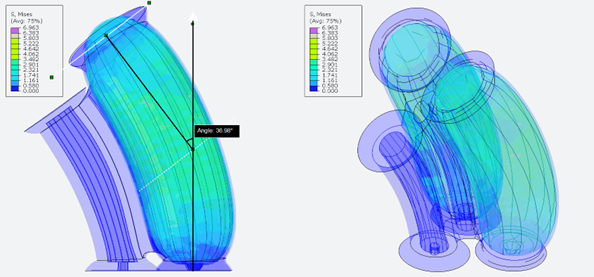
\includegraphics[align=c, scale=0.75]{d15}\\
	\hline
	6 & 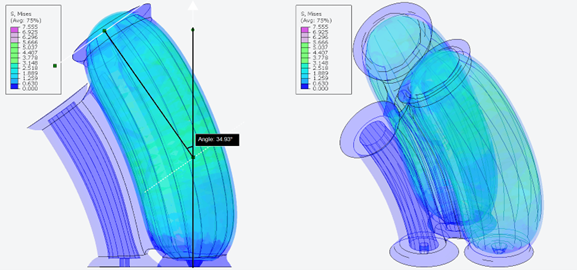
\includegraphics[align=c, scale=0.75]{d16}\\
	\hline
	\end{tabular}
	\caption{- The maximum angle the silicon parts can reach. 14mm version has the largest angle}
\end{table}

\todo{More tests regarding the extension of all parts. }
%------------------------------------------------
\section{Construction}

\subsection{Overall Structure}
As mentioned, the structure is designed intentionally to be modular, meaning that the length of the robot can be adjusted depending on the need. This also helps with maintenance as parts can be easily replaced. At the end, the final impletemented design is as follows. The front has an OpenMV module attached and then each segment follows is identical. Tubing for air runs along the snake and whether the chamber inflates or not is controlled by air valves placed at the entrance of the chamber. The silicon body is connected using acrylic sheets pushed together. The chambers are placed in a triangular pattern with a hold in the middle for wires and tubing. This shape provides stability and functionality. The top has one chamber to push down the robot for better friction and contact while two chambers on the bottom control turning. The robot is propped on fixed rubber wheels to add friction and reduce wear on the acrylic and silicon parts. 

\begin{figure} [H]
	\centering
	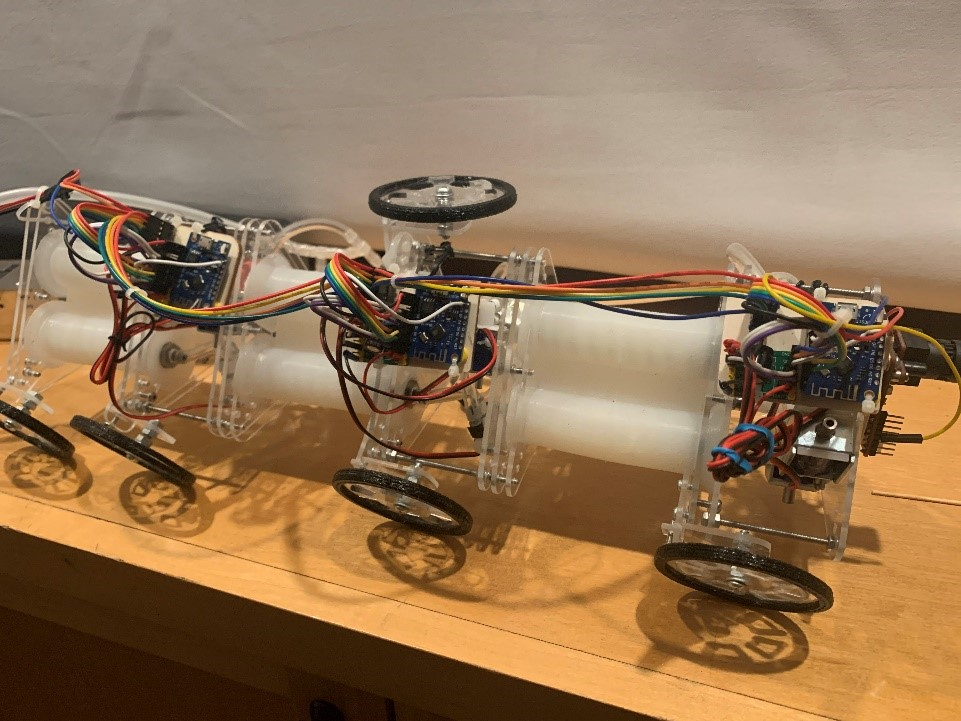
\includegraphics{completed_snake}
	\caption{Three segments of the robot wired together}
\end{figure}

\subsection{Tools}
Throughout the design of the structures, I relied heavily on a few tools. First is the designing tools. For CAD, I used a combination of Fusion 360, AutoCAD, and SolidWorks. Fusion 360 is used the most for general designs as it’s interface is simple and modern. I used AutoCAD to design two-dimensional sketches which are then sent to the CNC router. I used SolidWorks for assembling the different components of the snake together to check for interferences and oversights in the designs. 

These designs are then brought to reality with one of the two manufacturing processes. The first being FDM (Fused Deposition Modeling) 3D printing. Most of the 3D printed parts are with the 1.75mm PLA filaments as it is 100\% biodegradable and biosourced. It is also easy to print with and nontoxic like ABS, another popular choice of material. The other method is with a CNC router. All acrylic sheets are processed with a single flute flat end mill.

I also used both Fritzing and Altium Designer for presentation of circuit diagrams and SMCDraw for the pneumatics circuit diagram.

\begin{figure}[H]
	\centering
	
	\begin{minipage}{0.4\linewidth}
		\centering
		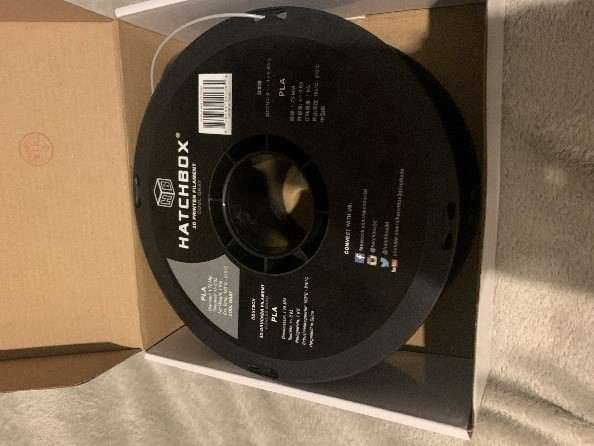
\includegraphics[width=\textwidth, angle=-90]{pla}
		\caption{HatchBox Gray 1.5mm PLA Filament I used}
	\end{minipage}
	\hfill	
	\begin{minipage}{0.4\linewidth}
		\centering
		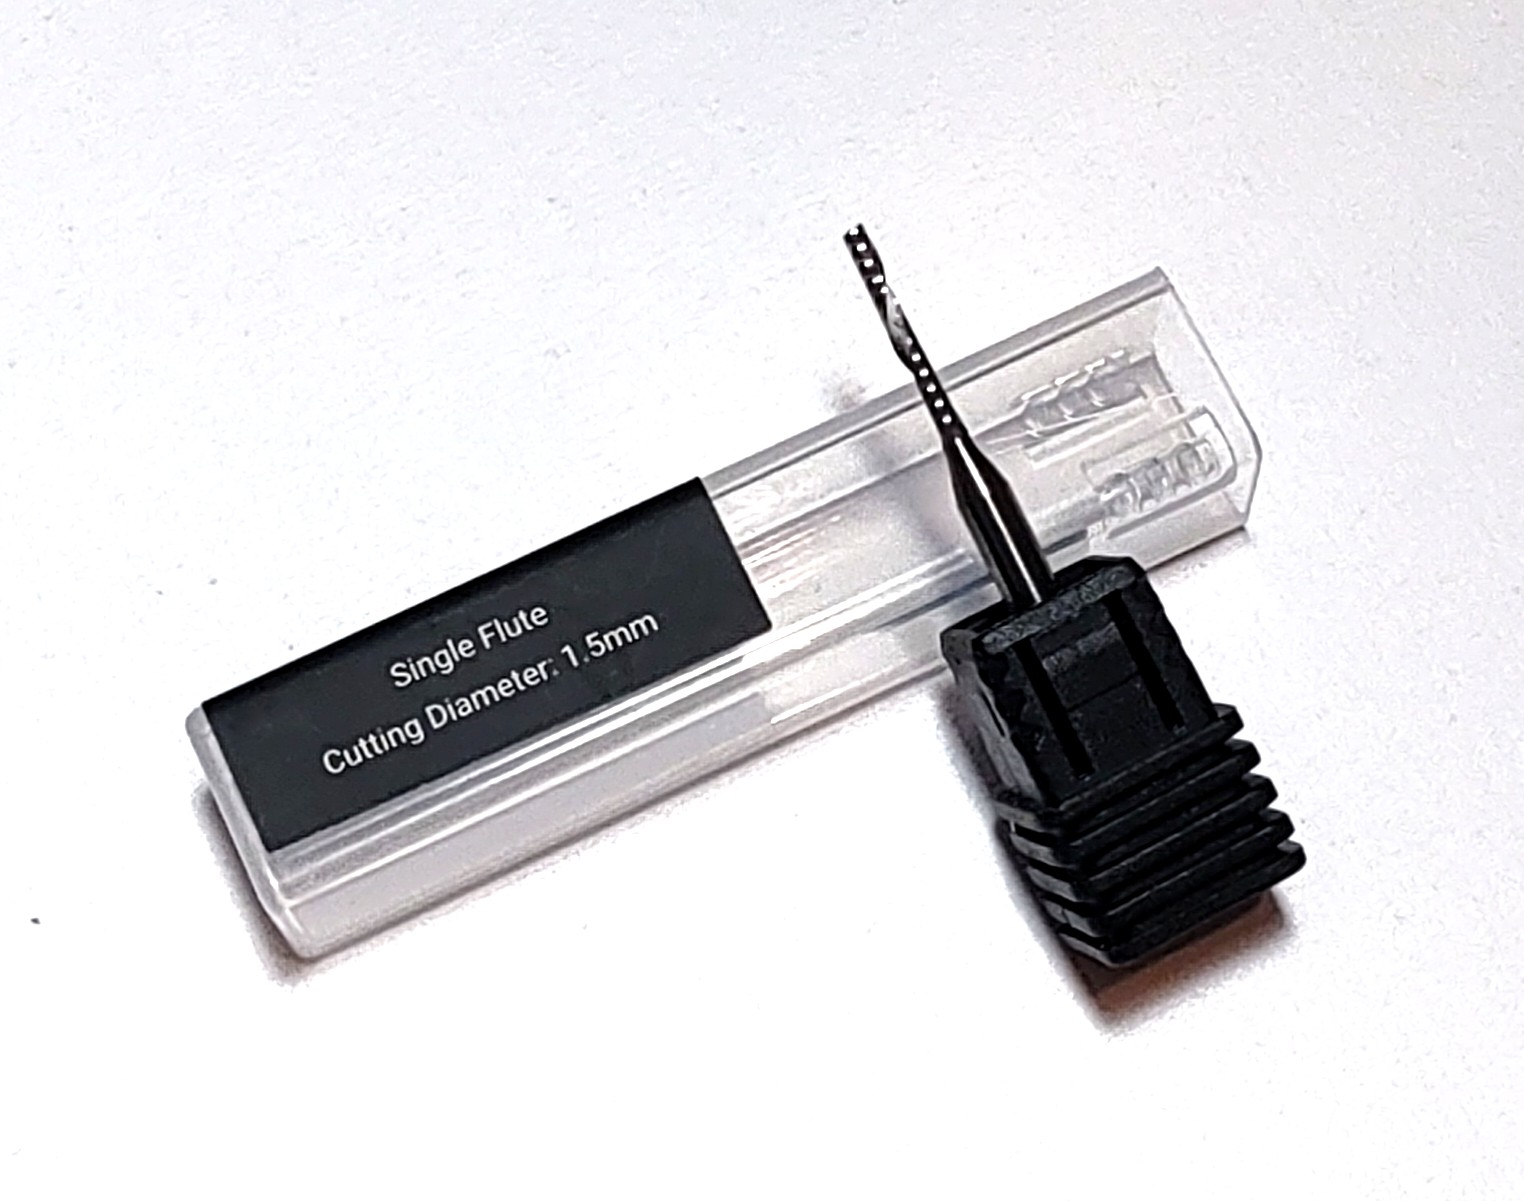
\includegraphics[width=\textwidth]{mill_bit}
		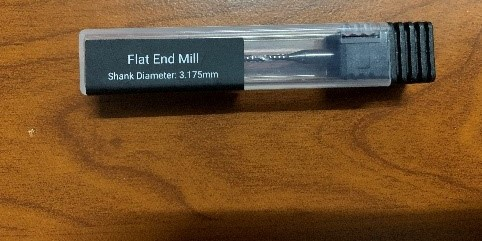
\includegraphics[width=\textwidth]{mill_bit_closed}
		\caption{Single Flute Flat End Mill with a cutting diameter of 1.5mm}
	\end{minipage}
\end{figure}

\subsection{Silicon Casting}
\blindtext
\todo{add description of the casting process and add images}
\subsection{Silicon Mold Revisions}
Each part of the robot has gone through multiple iterations. Especially the components related to the silicon body. 

The first version used wooden sticks which have a diameter of 12mm and springs with a diameter of 14mm. The smaller circle at the bottom is used to secure the wooden stick while the outer ring is used to hold the spring. The cutouts are used to hold the M3 hex nut. There are a total of three cutouts located near the top of the bottom part. Respectively, there are three through holes on each part that matches up. They are the holes for the M3 screws. Screws are used in this mold to apply pressure to the seam to minimize the silicon from leaking. However, this proved to be unnecessary as the fit can be tight enough to contain the silicon when the right amount of tolerance is applied. There is a ring of silicon both on the bottom and the top of the mold. This is to make sure that the acrylic plates can secure the silicon in place without it detaching.


\begin{figure}[H]
	\centering
	\begin{subfigure}[b]{0.33\linewidth}
		\centering
		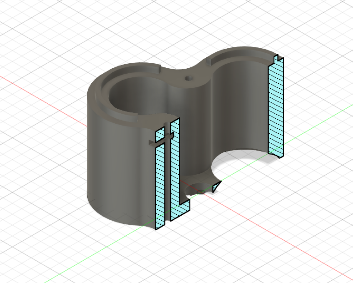
\includegraphics[width=\textwidth]{top_v1}
		\subcaption{Top CAD with Cross Section}
	\end{subfigure}%
	\begin{subfigure}[b]{0.33\linewidth}
		\centering		
		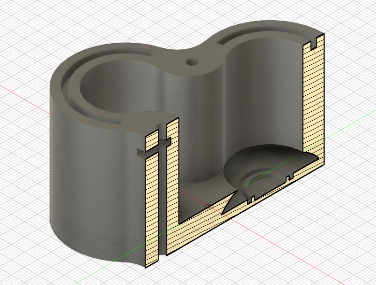
\includegraphics[width=\textwidth]{bottom_v1}
		\subcaption{Bottom CAD with Cross Section}
	\end{subfigure}%
	\begin{subfigure}[b]{0.33\linewidth}
		\centering
		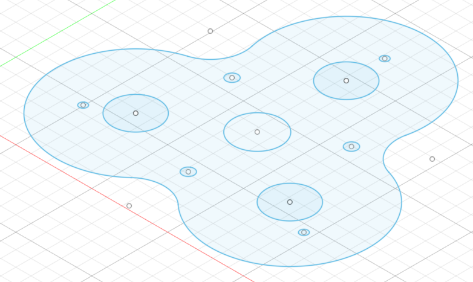
\includegraphics[width=\textwidth]{plate_cad}
		\subcaption{Plate CAD route}
	\end{subfigure}
	
	\begin{subfigure}[b]{0.33\linewidth}
		\centering
		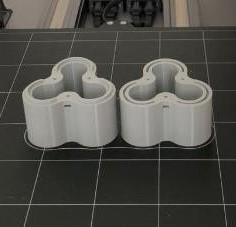
\includegraphics[width=\textwidth]{top_bottom_printed}
		\subcaption{Top and Bottom Printed}
	\end{subfigure}%
	\begin{subfigure}[b]{0.33\linewidth}
		\centering		
		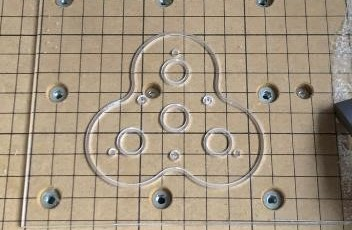
\includegraphics[width=\textwidth]{cover_plate_cnc}
		\subcaption{Cover Plate cut with CNC}
	\end{subfigure}%
	\begin{subfigure}[b]{0.33\linewidth}
		\centering
		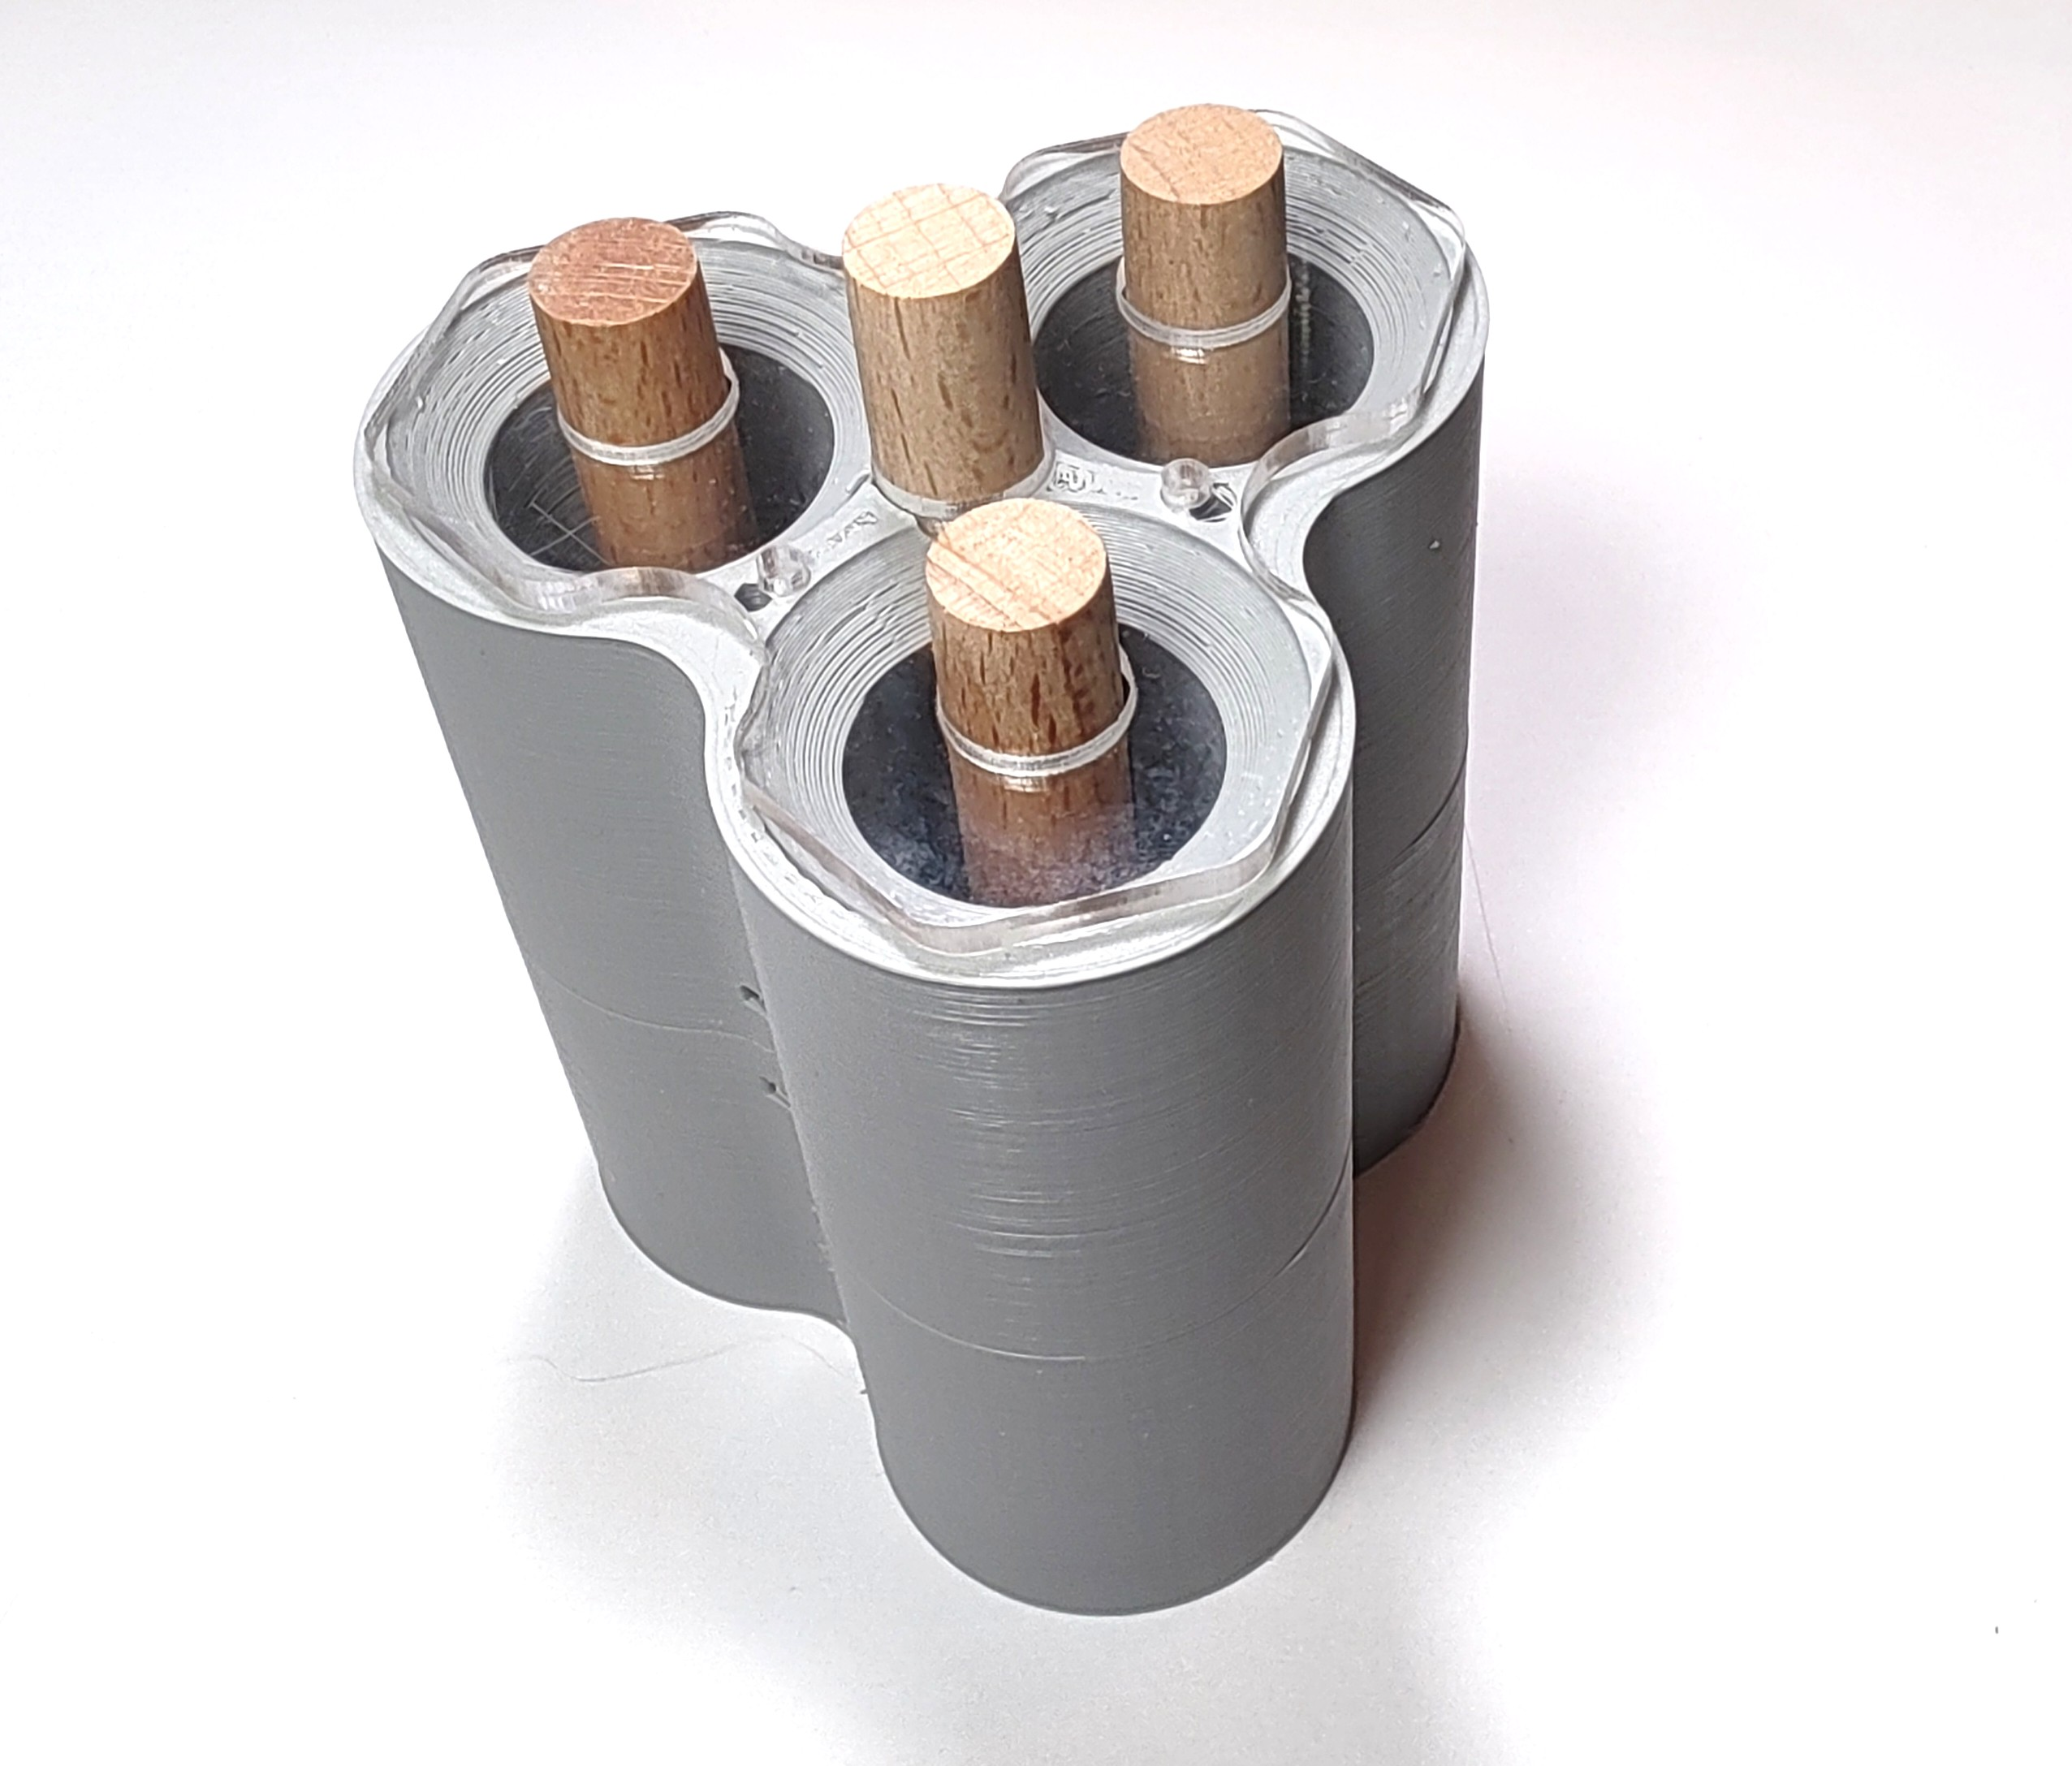
\includegraphics[width=\textwidth]{assembled_v1}
		\subcaption{the mold assembled}
	\end{subfigure}%
	\caption{Version 1 of the Mold}
\end{figure}

There are a few issues with this version. First, the use of the wooden stick meant that the size of the inner hole was unchangeable. This is especially problematic for experimenting with different wall thicknesses. Another issue was the sealed top plate. This meant the bubbles from the silicon cannot escape and would be trapped at the top making the surface uneven. The ring of silicon also was proven too small to keep the part in place. Applying a small amount of force will separate the plates and the silicon part. Due to the density of the stick, the inner surfaces of the silicon part were also not aligned properly. 

To test a variety of wall thicknesses, a new bottom with fixed pillars that is 14mm in diameter is designed. The ring was also enlarged to make ensure the part is secured. Since the stick no longer needs to be held in place by the plate and the bottom, The top was also removed to make sure no bubbles are formed. This new version had larger pillars but since it was fixed onto the mold, they had to be destroyed to extract the silicon body. 

\begin{figure} [H]
\centering
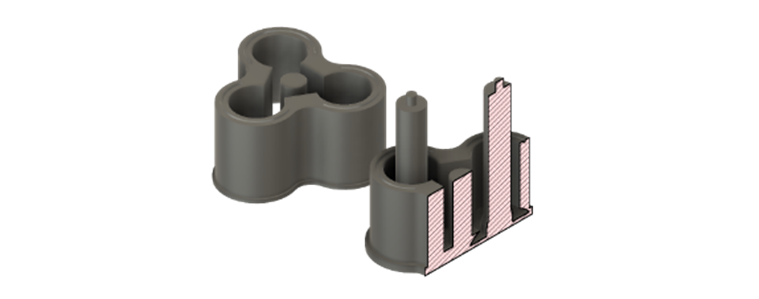
\includegraphics{mold v2}
\caption{Version 2 of the mold. The stick is attached to the base, which made the removal of the mold from the silicon impossible}
\end{figure}

The third version redesigned the bottom so that the walls and the base detach. This means that the pillars and the base can be pulled out before removing the silicon body. Although the base was still difficult to remove, it can now be used multiple times. During the tests, it was also proven that the seal between the acrylic plates securing the silicon part and the silicon was too weak to withstand high pressures. Therefore, another silicon mold was added to create a thin layer of silicon that will be glued to the end to ensure an air-tight seal. 

\begin{figure} [H]
\centering
\begin{subfigure}[b]{0.5\linewidth}
		\centering
		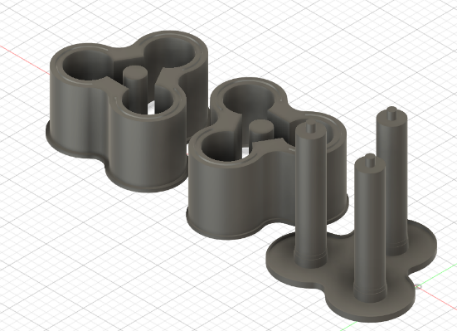
\includegraphics[width=\textwidth]{mold_v3}
		\subcaption{Version 3 of the mold with a new detachable base}
	\end{subfigure}%
	\begin{subfigure}[b]{0.5\linewidth}
		\centering		
		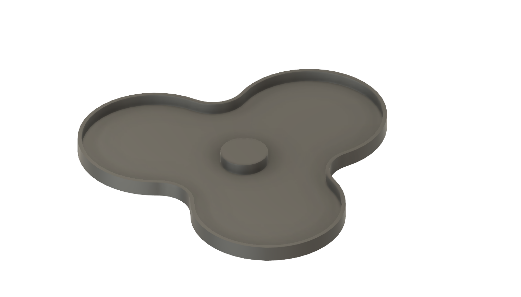
\includegraphics[width=\textwidth]{sealing_v3}
		\subcaption{Newly added mold for sealing}
	\end{subfigure}
\caption{Version 3 of the mold}
\end{figure}

However, gluing two silicon parts together soon proved weak. It cannot contain the amount of pressure needed to move the snake. Therefore, a new mold is designed. This one allowed the silicon to be molded all at once and it only had one opening which is for the valve and the input for air. It flipped the orientation of the silicon part in the mold upside-down as now the only opening is now facing down. The pillars are now independent from the base and is secured by the hole in the bottom plate. The silicon part will be first removed from the mold with the pillars and then the pillars will be pulled out.

\begin{figure} [H]
\centering
\begin{subfigure}[b]{0.5\linewidth}
		\centering
		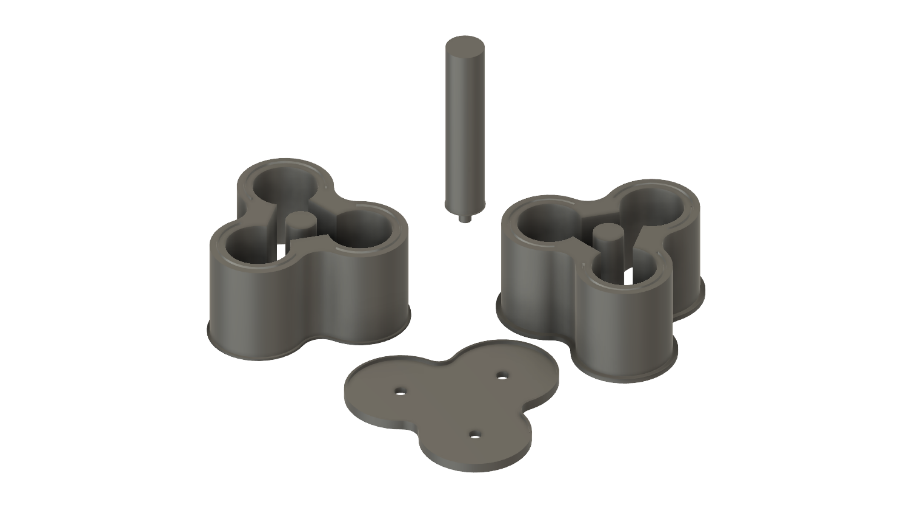
\includegraphics[width=\textwidth]{mold_v4}
		\subcaption{Version 4 of the mold with detachable pillars}
	\end{subfigure}%
	\begin{subfigure}[b]{0.5\linewidth}
		\centering		
		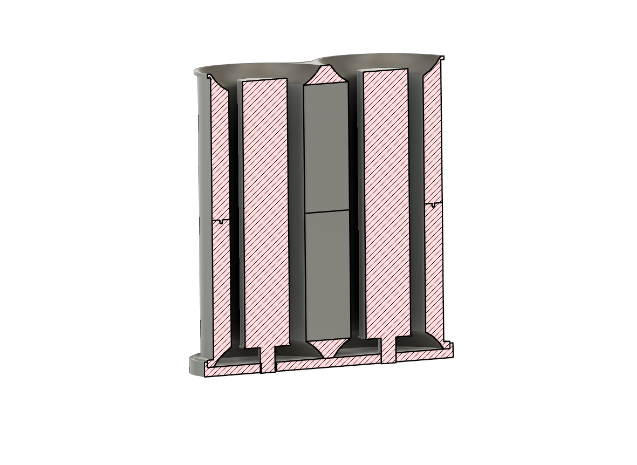
\includegraphics[width=\textwidth]{assembled_v4}
		\subcaption{Assembled Mold}
	\end{subfigure}
\caption{Version 4 and the final version of the mold}
\end{figure}

\subsection{Communication Protocol}
Although it was established that the segments are going to be designed with the idea of modularity, the actual approach changed. The first iteration was using ESP8266 as a microcontroller for each segment, and there will be one for each segment. They will be connected using I2C and instructions are going to be sent from the OpenMV module at the front. However, after some research and experiment, it was concluded that although labeled with such a feature, ESP8266 doesn’t support receiving I2C. Thus, the protocol was switched to Serial, which provides similar functionality but requires me to program my own communication protocols while I2C has this functionality packaged already.

\subsection{Airway}
There is one overall air pump that sends air through the clear PVC tubing, and this pump is capable of exerting 12kPa. The air from the pump is them separated into tubing for each segment and then each solenoid valve. The valve tubing is then connected to a custom-printed valve core that ensures an air-tight seal between the tubing and the silicon chamber. There are two states of the solenoid valve and when it is powered, the air flows into the silicon chamber, and when the valve is not powered, the air flows out from the chamber. When the top and the left solenoid valve is powered, the air flows into those two chambers and bents this segment towards the right and when the top and the right solenoid valve are powered, the segment bends left. 

\begin{figure}[H]
	\centering
	\begin{subfigure}[b]{0.33\linewidth}
		\centering
		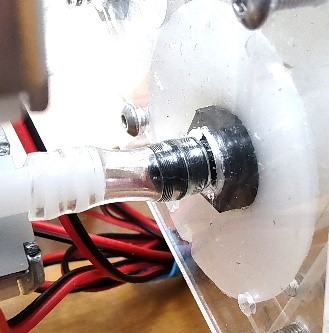
\includegraphics[width=\textwidth]{air_connection}
		\subcaption{Top CAD with Cross Section}
	\end{subfigure}%
	\begin{subfigure}[b]{0.33\linewidth}
		\centering		
		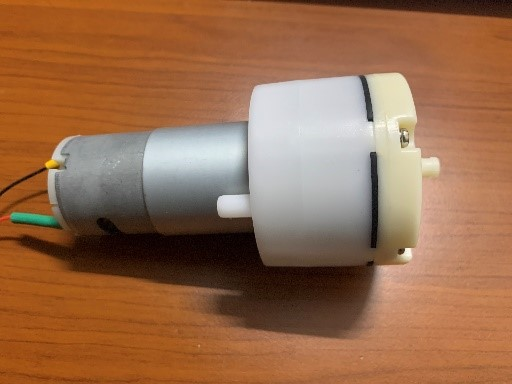
\includegraphics[width=\textwidth]{air_pump}
		\subcaption{Bottom CAD with Cross Section}
	\end{subfigure}%
	\begin{subfigure}[b]{0.25\linewidth}
		\centering
		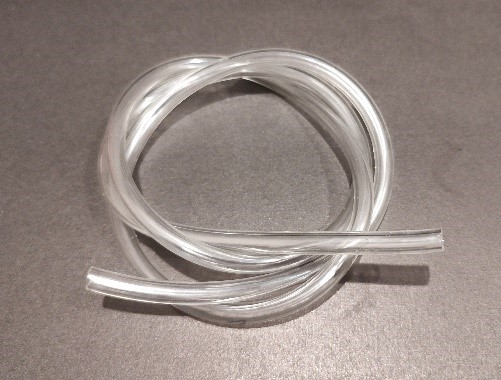
\includegraphics[width=\textwidth]{pvc_tubing}
		\subcaption{Plate CAD route}
	\end{subfigure}
	
	\begin{subfigure}[b]{0.33\linewidth}
		\centering
		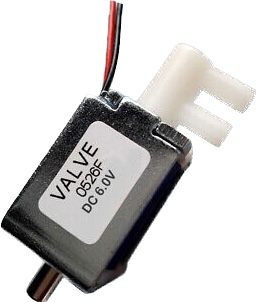
\includegraphics[width=\textwidth]{solenoid valve}
		\subcaption{Top and Bottom Printed}
	\end{subfigure}%
	\begin{subfigure}[b]{0.33\linewidth}
		\centering		
		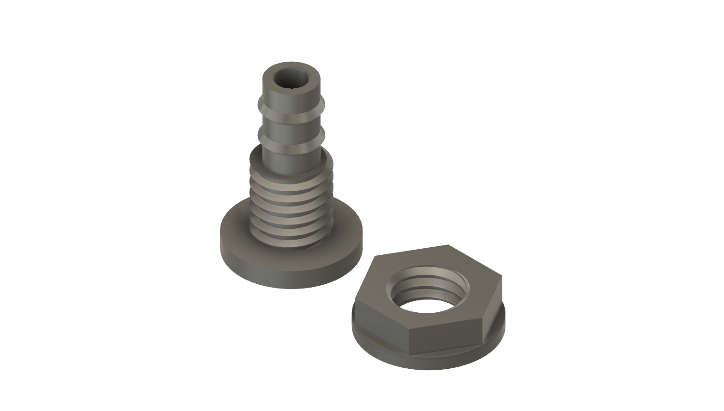
\includegraphics[width=\textwidth]{valve}
		\subcaption{Cover Plate cut with CNC}
	\end{subfigure}%
	\begin{subfigure}[b]{0.33\linewidth}
		\centering
		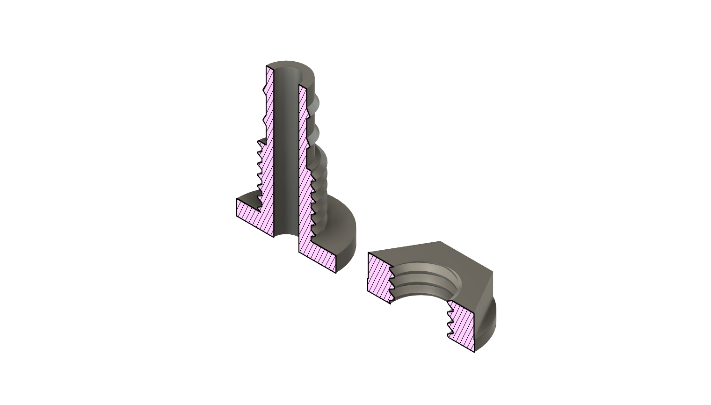
\includegraphics[width=\textwidth]{valve_section}
		\subcaption{the mold assembled}
	\end{subfigure}%
	\caption{Version 1 of the Mold}
\end{figure}

\begin{figure} [H]
	\centering
	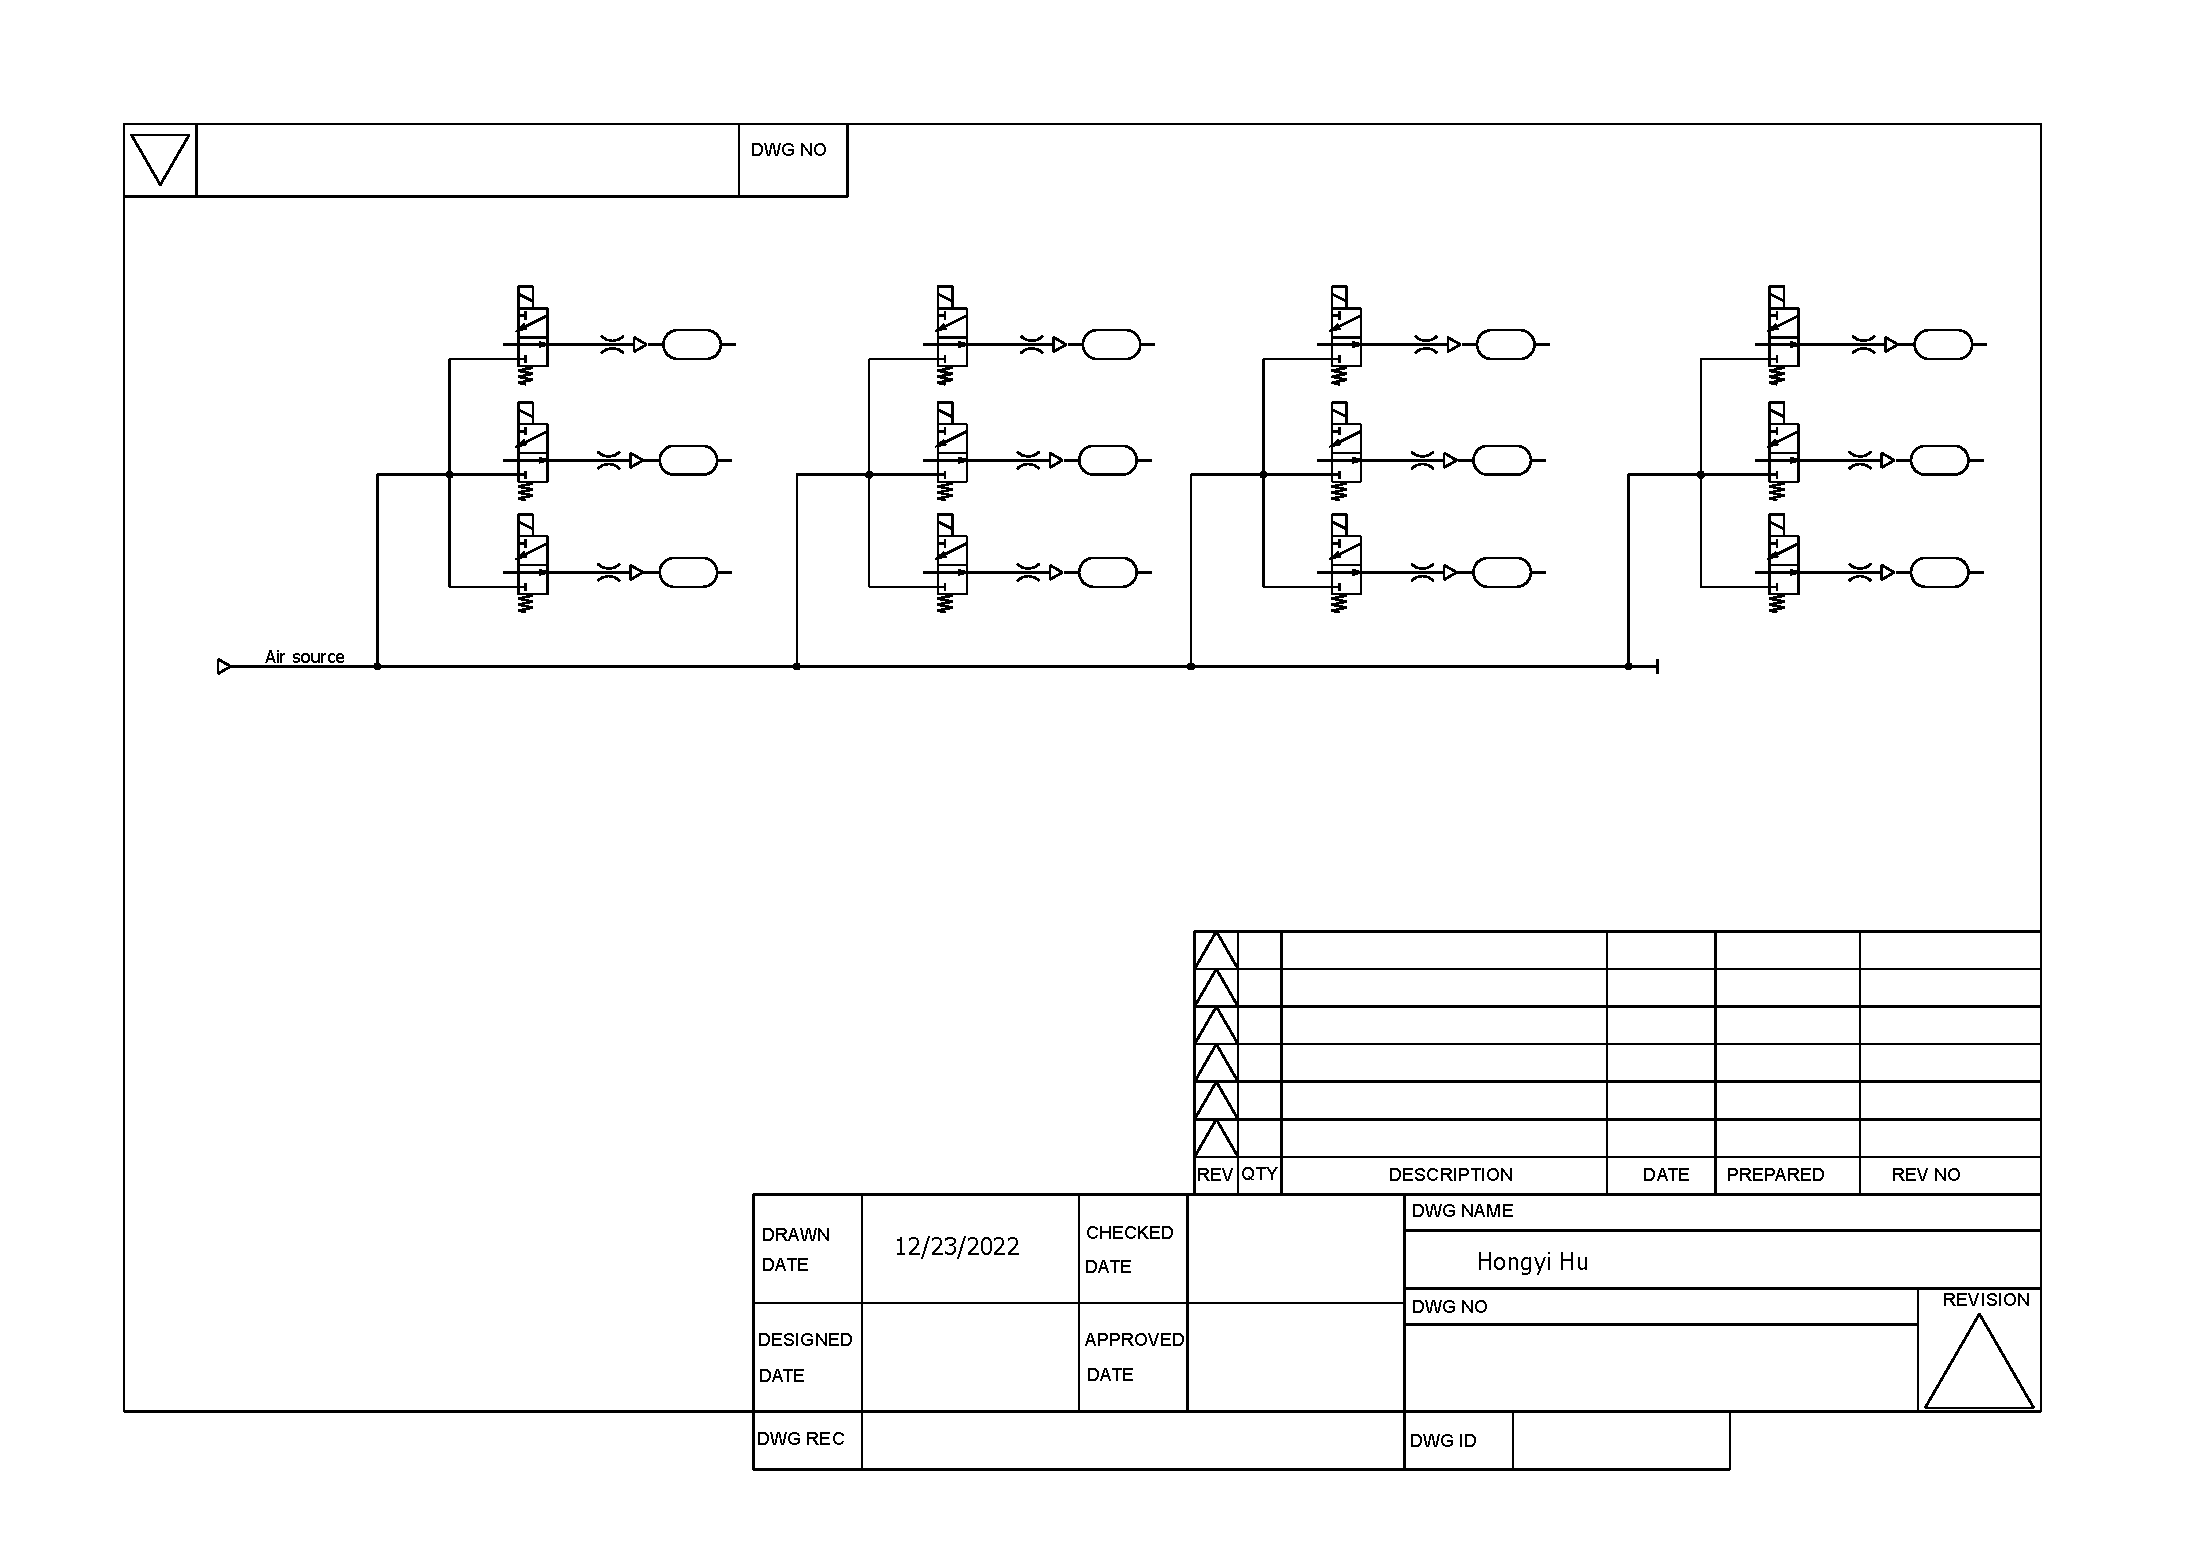
\includegraphics[width=\linewidth]{pneumatic circuit design}
	\caption{Pneumatic Circuit design of four segments of the snake}
\end{figure}

\subsection{Change to Standoffs}
The actual structure differed from the design in the connecting pieces. The original designed used brass standoffs of various lengths while the actual structure made use of long bolts. This is because the longs screw allows for finer adjustments that the brass standoffs cannot provide, and this is especially important during prototyping phase as changes are made frequently. 

\subsection{Wheels}
At firs the wheel is just the acrylic cutout, but the acrylic wheel provided poor friction and was not enough to push the robot forward. Thus, I 3d printed some grooved wheels with a TPU filament. TPU is a soft and flexible material which the most ideal material to be used to 3D print a wheel as it is easier to print compared to other flexible materials while still offer a good coefficient of friction. 

\begin{figure}[H]
	\centering
	\begin{subfigure}[b]{0.5\linewidth}
		\centering
		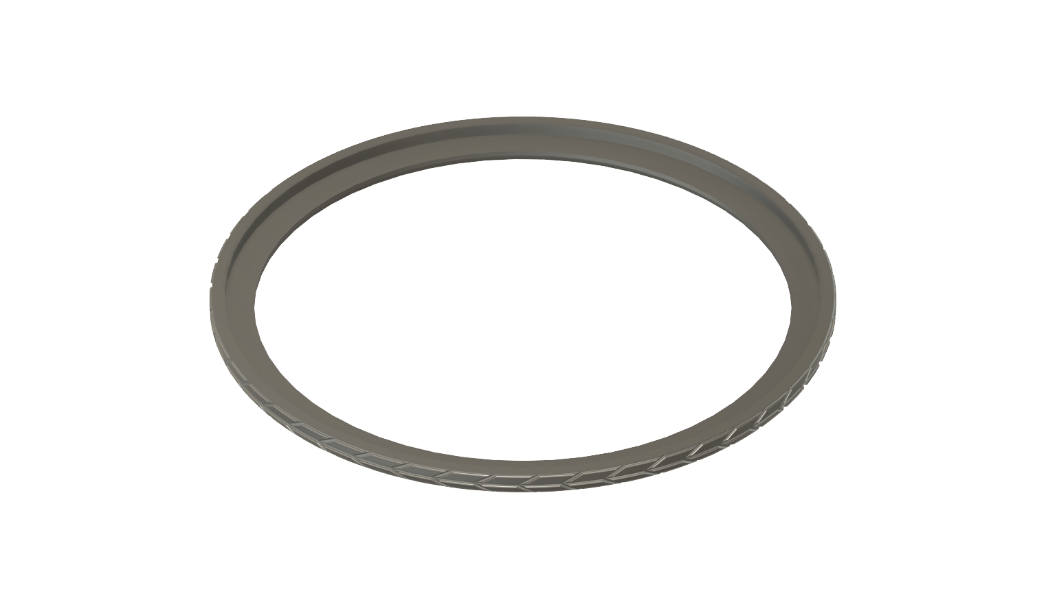
\includegraphics[width=\textwidth]{half_tire_cad}
		\subcaption{CAD of half of the tire}
	\end{subfigure}%
	\begin{subfigure}[b]{0.5\linewidth}
		\centering		
		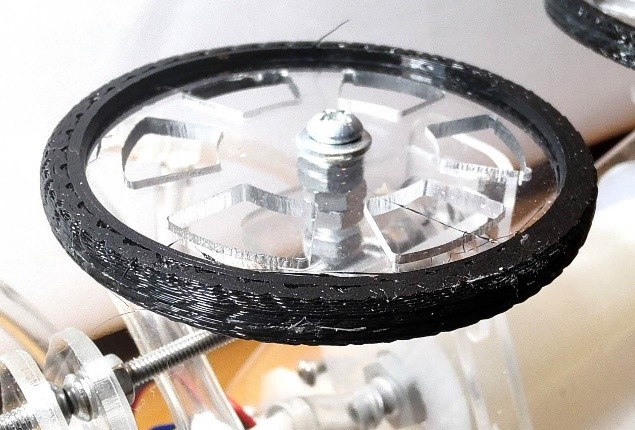
\includegraphics[width=\textwidth]{full_tire}
		\subcaption{Two halves of the tire glued together to the acrylic rim}
	\end{subfigure}
	\caption{Tires used in the robot}
\end{figure}

%------------------------------------------------

\section{Electrical Design}

The OpenMV at the front of the robot is used for image recognition as well as for sending signals to each segment and controlling the movement of the robot. It is programmed in micro-Python. This allows for simpler code as well as the possibility to add AI recognition through OpenCV to the robot. Each ESP8266 is a receiver for the commands and a controller of the three solenoid valves on a segment, which controls whether then controls the flow of the air. ESP8266 can be coded in Arduino and is feature packed. Although right now each segment is connected through UART, the on-board Wi-Fi module allows the possibility to communicate via Wi-Fi with the other modules in the future. The ESP8266 is connected to an A4950 motor drive which is then connected to the solenoid valves. 

\todo{add figures of actual parts and explain functionality}

\begin{figure} [H]
	\centering
	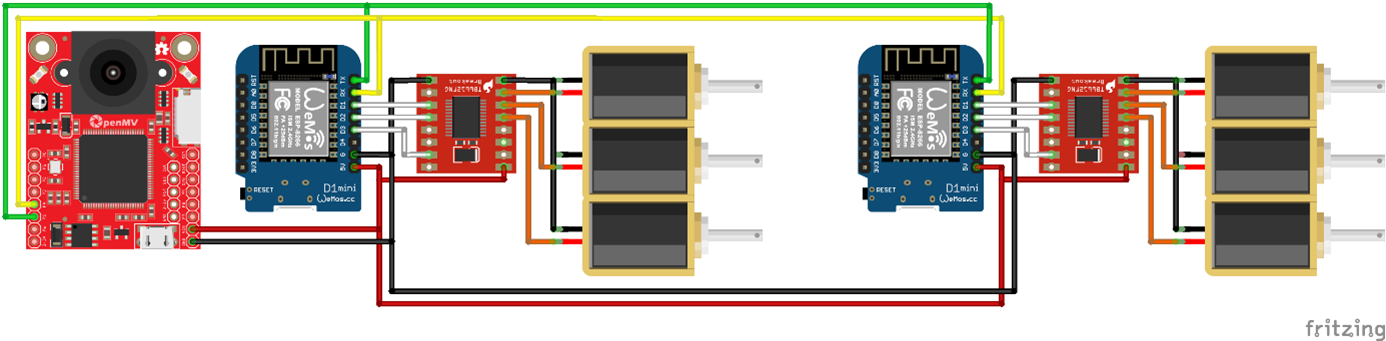
\includegraphics[width=\linewidth]{wiring_diagram}
	\caption{Wiring Diagram of the snake}
\end{figure}
\begin{figure} [H]
\centering
	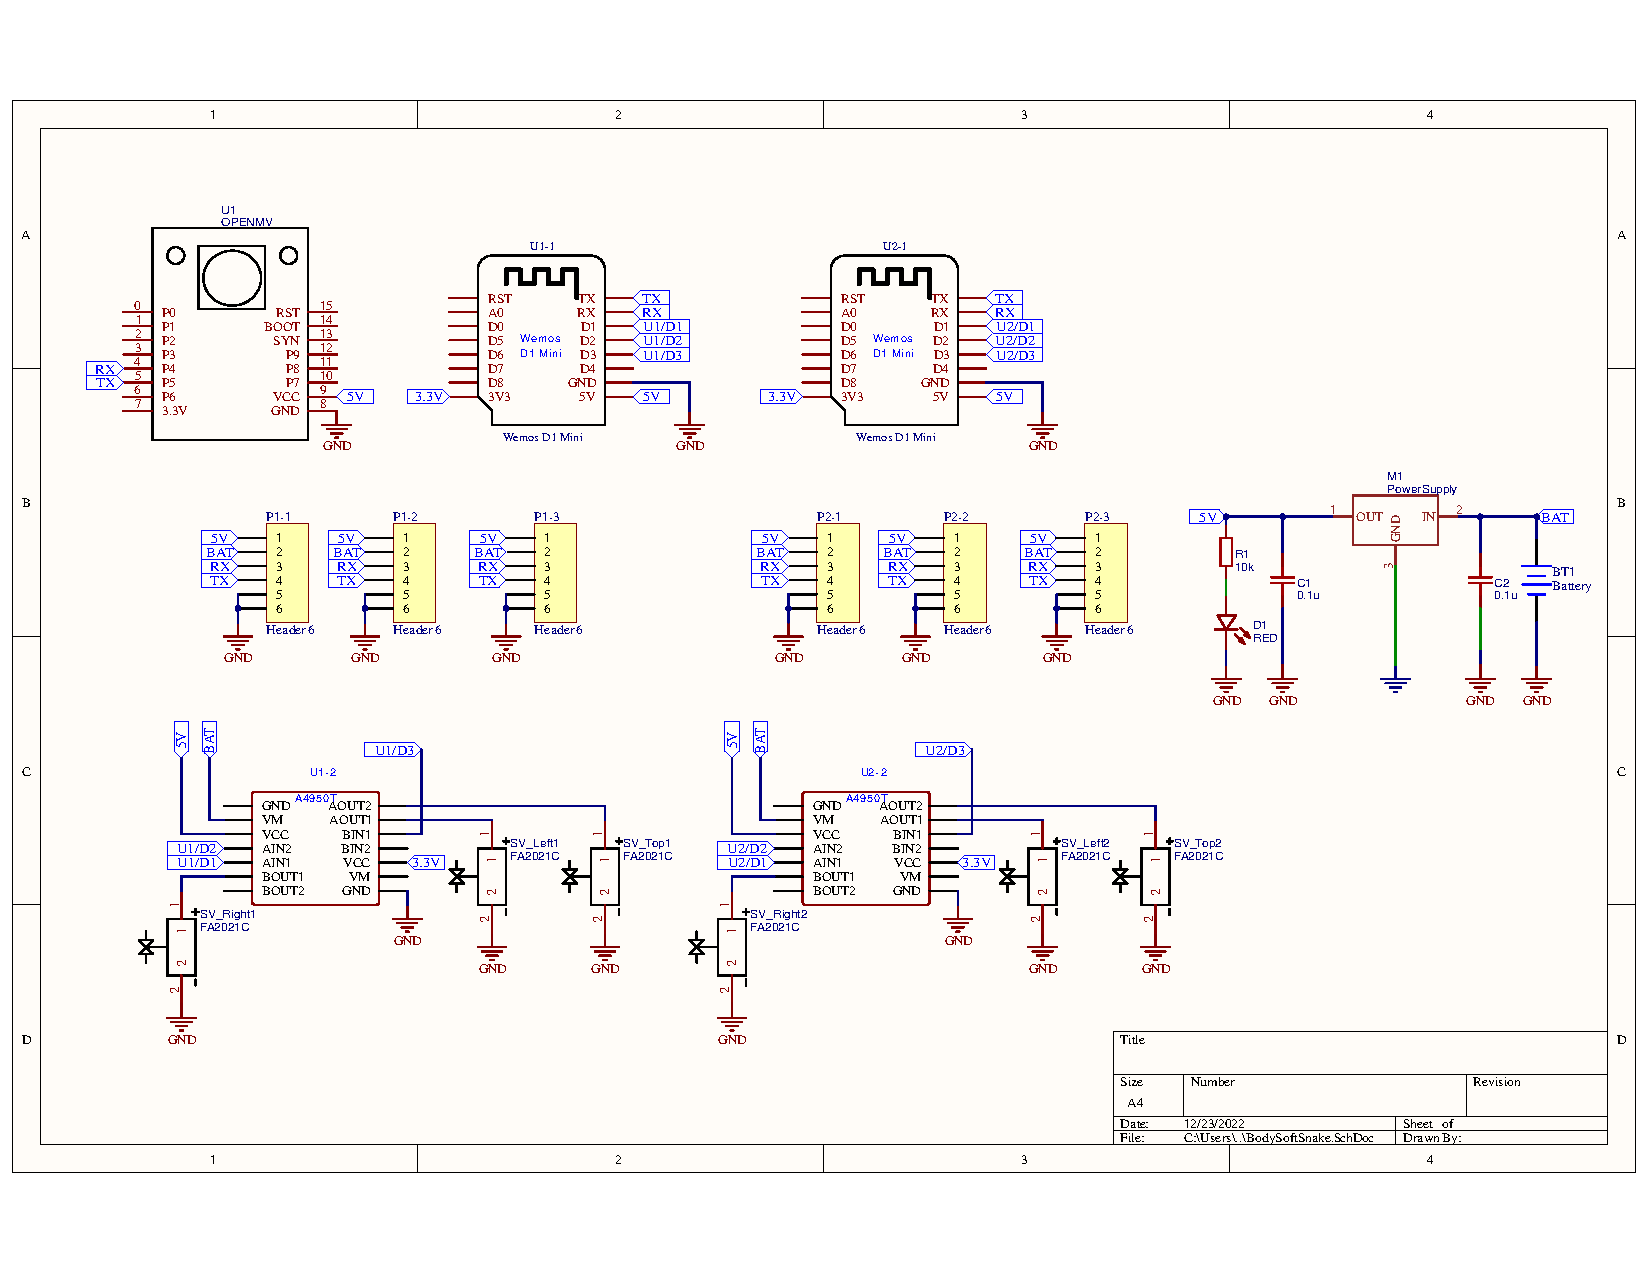
\includegraphics[width=\linewidth]{electric circuit diagram}
	\caption{Wiring Diagram of the snake}
\end{figure}

\section{Software Design}
There are two movement types that the robot can perform depending on the environment and they all drew inspiration from the movements of a real snake. The serpentine locomotion is best for general purposes when there is a lot of open space. It is the S-shape movement people normally associate with snakes. The other type is concertina locomotion. This is best suited for tighter spaces where the snake cannot perform serpentine locomotion. It curls its tail while keeping the front stationery, and then keeps its tail stationary and extends its front. This repetition of curling and extending allows the snake to travel at narrow pathways. Each of these is achieved by predefined controls in the front OpenMV. There are two controls currently. The first is manual, where the user can directly control the movement of the snake. The second is automatic, where the snake will use its front-facing camera to follow a certain object. Regardless of which method, the openMV module converts the desired locomotion into a series of movements each segment performs and is distributed to each ESP8266. Since they relate to the same Serial port, a package header with an address that is unique to each segment is attached to the beginning of the command to assign this instruction to a specific segment. 

\begin{table}[H]
\centering
\begin{tabular}{|c|c|c|}
\hline
Name & Purpose & Size \\\hline
Header & Signals which segment this command is for & 1 byte\\\hline
Instruction & A code that tells ESP8266 which action to perform & 1 byte\\\hline
\end{tabular}
\caption{Structure of the packages send out by the OpenMV to each ESP8266}
\end{table}

Althuogh the size of the package could be further decreased by using a nibble to represent each component (15 different addresses can be represented by a nibble not counting 0000, and technically only 2 bits are needed to represent the command), resulting in a much smaller packag, it is hardly necessary because the speed to UART3 is fast enough and the number of packages are few enough that a 2-byte-sized package will not hinder the performance. 

The OpenMV first initializes the UART and the state of each segment to 0, which represents a neutral, straight segment, except for the first segment, which is set to -1, which represents a segment curved to the right. Similarly, the number 1 represents a segment curved to the right. Then, the program checks for the locomotion. If the mode is serpentine, the the program updates the state of each segment to that of the segment in front of. After updating all segments including the first segment which is updated seperately as there is no segments in front, the new state is then converted into a char that represents the command after which will result in the desired state. The OpenMV first sends the address of the segment that should recieve this instruction and then follows it by the actual instruction. It does so for every segment, and then waits for the predefined amount of time, which is how long it takes to fully inflate the silicon chambers. After inflation, the state of the segment is updated again.

\begin{figure} [H]
	\centering
	\hspace*{3cm}%
	\begin{tikzpicture}[node distance=2cm, auto]
		\node (start) [startstop] {Start};
		\node (pro1) [process, below of=start] {Initialize state of each segment};
		\node (dec1) [decision, below of=pro1, yshift=-0.5cm] {Locomotion};
		\node (dec2b) [decision, below of=dec1, yshift=-1cm] {Direction};
		\node (dec2bb) [process, right of=dec2b, node distance=4cm, yshift=-1cm]{Reverse\\ segment\_addr list};
		\node (pro2ba) [process, below of=dec2b, yshift = -0.5cm]{change inflation state for each segment};
		\node (pro3ba) [process, below of=pro2ba]{change inflation state for each segment};
		\node (pro4ba) [io, below of=pro3ba]{send package to\\ every segment};
		\node (pro5ba) [process, below of=pro4ba]{wait for chambers to inflate};
	
		\draw [arrow] (start) -- (pro1);
		\draw [arrow] (pro1) -- (dec1);
		\draw [arrow] (dec1) -- node[anchor=west] {Serpentine} (dec2b);
		\draw [arrow] (dec2b) -- node[anchor=west] {Forward} (pro2ba);
		\draw [arrow] (dec2b) -| node[anchor=south, xshift=-1cm] {Backward} (dec2bb);
		\draw [arrow] (dec2bb) |- (pro2ba);
		\draw [arrow] (pro2ba) -- (pro3ba);
		\draw [arrow] (pro3ba) -- (pro4ba);
		\draw [arrow] (pro4ba) -- (pro5ba);
	
		\node (c1) [coord, on grid, left of=pro5ba, node distance=1.5cm, xshift=-1cm] {};
		\draw [arrow] (pro5ba) -- (c1) |- (pro2ba);
	\end{tikzpicture}
	\caption{Flow chart how the front OpenMV commands each segment}
\end{figure}

Upon recieving a new byte data from the UART, each segment checks if the address matches that of itself. If it does not, then it will still read the next byte but will not process it in order to be ready to read the next header. If the address does match, then it will read the next instruction and perform the corresponding action. If character "S" is sent through, the segment will unpower all solenoid valves to release all chambers and have the silicon part return to neutral position. If "L" is sent through, the top and right solenoid valve will close and those two chambers will inflate, making the segment curve to the left. Similarly, if the instruction is "R", the top and left solenoid valve will close so the segment curves to the right. 

\begin{figure}[H]
	\centering
	\hspace*{-0.5cm}%
	\begin{tikzpicture} [node distance=2cm, auto]
		\node (start) [startstop, xshift=8cm] {Start};
		\node (dec1) [decision, below of=start, yshift=-0.5cm] {check for packages};
		\node (dec2) [decision, below of=dec1, yshift=-1cm] {check header};
		\node (dec3) [decision, below of=dec2, yshift=-1cm] {read instruction};
		\node (pro4a) [process, below of=dec3, node distance=2.25cm] {stop powering all solenoids};
		\node (pro4b) [process, left of=pro4a, node distance=4cm] {power top + right solenoid};
		\node (pro4c) [process, right of=pro4a, node distance=4cm] {power top + left solenoid};
		\node (io3) [io, left of=dec2, xshift=-2cm, yshift=1.5cm] {read header}; 
		\draw [arrow] (start) -- (dec1);
		\draw [arrow] (dec1) -- node {new pacakge} (dec2);
		\draw [arrow] (dec2) -- node {for this segment} (dec3);
		\draw [arrow] (dec3) -- node {"S"} (pro4a);
		\draw [arrow] (dec3) -| node[anchor=south, xshift=1cm] {"L"} (pro4b);
		\draw [arrow] (dec3) -| node[anchor=south, xshift=-1cm] {"R"} (pro4c);
		\node (c1) [coord, on grid, right of=dec1, xshift=1cm] {};
		\draw [arrow] (dec1) -- (c1) |- node [anchor=south,xshift=-1.5cm] {no new pacakge} (dec1.north);
		\draw [arrow] (dec2) -| node[anchor=north, xshift=0.5cm]{not for segment}(io3);
		\draw [arrow] (io3) |- (dec1.north);
		
		\node (c2) [coord, on grid, below of=pro4b, xshift=-3cm, yshift=1cm] {};
		\draw [arrow] (pro4b) |- (c2) |- (dec1.north);
		\draw [arrow] (pro4a) |- (c2) |- (dec1.north);
		\draw [arrow] (pro4c) |- (c2) |- (dec1.north);
	\end{tikzpicture}
	\caption{Flow chart of how each segment functions}
\end{figure}

\section{Tests}
\blindtext
\todo{add some actual tests performed, success, failure, single module test, result analysis, reason, insert images of video}

\section{Conclusion}
This project did not achieve everything planned at the beginning. It only achieved the basic function of the robot, yet it is lacking a lot of software to support it. The implementation of an AI image recognition system is crucial as well as a purely image-based mapping system is also yet to be done. A coordinate system is also necessary to know the actual location of the snake. Without these, the robot cannot achieve its full potential as a life-saving device. Apart from the software, the silicon body design will also need to be improved as the current design does not make use of the pull potential of the air pressure.



%----------------------------------------------------------------------------------------
%	REFERENCE LIST
%----------------------------------------------------------------------------------------

\begin{thebibliography}{99} % Bibliography - this is intentionally simple in this template

\bibitem[Figueredo and Wolf, 2009]{Figueredo:2009dg}
Figueredo, A.~J. and Wolf, P. S.~A. (2009).
\newblock Assortative pairing and life history strategy - a cross-cultural
  study.
\newblock {\em Human Nature}, 20:317--330.
 
\end{thebibliography}

%----------------------------------------------------------------------------------------

\end{document}
